\section{Implementaci\'on}
\label{sec:Implementacion}
    % Parrafo 1
        Como mencionamos en el Marco Te\'orico, nos centraremos en el simulador del 
            Physarum Polycephalum y en el robot con una Raspberry Pi. En este caso,
            el simulador del Physarum Polycephalum se encargar\'a de determinar la ruta
            \'optima para recolectar informaci\'on de la poblaci\'on. Por otro lado, el
            robot con una Raspberry Pi se encargar\'a de recolectar informaci\'on de la
            poblaci\'on y de los entornos en los que se encuentran.
        \vskip 0.5cm
    % Parrafo 2
        En este cap\'itulo, se detallar\'a la implementaci\'on de estos sistemas. 
            Primero, se describir\'a la implementaci\'on del simulador del Physarum Polycephalum.
            Luego, se describir\'a la implementaci\'on del robot con una Raspberry Pi.
            Finalmente, se describir\'a la integraci\'on de estos sistemas.
        \vskip 0.5cm
    \subsection{Simulador del Physarum Polycephalum} % (fold)
\label{sub:subsection name}

    El algoritmo propuesto se basa en el descrito por Jeff Jones en su obra 
    'From Pattern Formation to Material Computation: Multi-agent Modelling of Physarum Polycephalum' \cite{Jones2015}.
    \vskip 0.5cm
    %P\'arrafo 2
    El algoritmo es un aut\'omata celular que simula el comportamiento de Physarum Polycephalum en un laberinto, por lo que necesitamos definir algunos conceptos.
        Primero, denotemos $\mathbb{Z}$ como el conjunto de enteros, es decir, $\mathbb{Z} = (-\infty, -1, 0, 1, \infty)$.
        y la longitud de cualquier tupla $x$ como $|x|$. Para todas las tuplas $x$ e $y$ de la misma longitud, denotemos $x \oplus y$
        como la tupla que resulta de la suma componente a componente de $x$ e $y$, es decir, $(x \oplus y)_i = x_i + y_i$ para todo
    $i \in \mathbb{Z}$.
    \vskip 0.5cm
    %P\'arrafo 3
    Entonces tenemos que un aut\'omata celular es una tupla $(\mathbb{Z}^{n}, S, N, f)$ tal que la dimensi\'on $n$ es al menos 1 donde 
        $n \in \mathbb{Z}^{+}$, $S$ es un conjunto finito y no vac\'io de estados, $N$ es un conjunto finito y no vac\'io de vecindarios 
        pertenecientes a $\mathbb{Z}^{n}$, y $f$ es una funci\'on de transici\'on local, es decir, $f: S^N \rightarrow S$ donde
        $S^N$ representa el conjunto de todas las configuraciones de vecindarios posibles en $N$.
    \vskip 0.5cm
    %P\'arrafo 4
    As\'i, el algoritmo propuesto en este trabajo se define como un aut\'omata celular $(\mathbb{Z}^{2}, S, N, f)$ donde $n = 2$, 
        $S = \{0, 1, 2, 3, 4, 5, 6, 7, 8\}$, $N = \{0, 1, 2, 3, 4, 5, 6, 7, 8\}^9$, 
        y $f : \{0, 1, 2, 3, 4, 5, 6, 7, 8\}^9 \rightarrow \{0, 1, 2, 3, 4, 5, 6, 7, 8\}$,\((C(x,y:t), N(x,y:t), M(x,y:t)) \) 
        representa el estado combinado, vecindario y memoria de la c\'elula en la posici\'on \((x, y)\) en el tiempo \( t \). La funci\'on de transici\'on 
        \( f \) se define como sigue:
    \begin{equation*}
    \begin{aligned}
    f(C(x,y:t), N(x,y:t), M(x,y:t)) = & \begin{cases}
        7 & \text{si } C(x,y:t) = 0 \text{ y } \exists N \in \{3, 4, 6\} \text{y } M(x,y:t) = 0 \\
        6 & \text{si } C(x,y:t) = 1 \text{ y } \exists N \in \{5, 6\} \\
        2 & \text{si } C(x,y:t) = 2 \\
        3 & \text{si } C(x,y:t) = 3 \\
        5 & \text{si } C(x,y:t) = 4 \text{ y } \exists N \in \{3, 5, 6\} \\
        & \text{y } M(x,y:t) = 0 \text{ y } N \not\in \{0, 7\} \\
        0 & \text{si } C(x,y:t) = 5 \text{ y } M(x,y:t) \not\in \{5, 8\} \\
        & \text{y } N \not\in \{1, 3, 4, 6\} \\
        8 & \text{si } C(x,y:t) = 5 \\
        & \text{ y la condici\'on anterior no se cumple} \\
        4 & \text{si } C(x,y:t) = 7 \text{ y } \exists N \in \{3, 4, 6\} \\
        5 & \text{si } C(x,y:t) = 8 \\
        1 & \text{si } C(x,y:t) = 1 \\
    \end{cases}
    \end{aligned}
    \end{equation*}
    %Tabla de estados
    Donde los estados del aut\'omata celular se definen en la \textbf{Tabla \ref{tab:estados}}.
    \vskip 0.5cm
    \begin{table}[h]
        \begin{center}
            \begin{tabular}{|c|c|c|}
                \hline
                \textbf{Color}&\textbf{Estado}&\textbf{Descripci\'on} \\
                \hline
                \cellcolor{blue} & 0 & Campo libre  \\
                \cellcolor{royalblue} & 1 & Nutriente no encontrado \\
                \cellcolor{red} & 2 & Repelente \\
                \cellcolor{black} & 3 & Punto inicial \\
                \cellcolor{yellow} & 4 & Gel contray\'endose \\
                \cellcolor{darkgreen} & 5 & Gel compuesto \\
                \cellcolor{lemon} & 6 & Nutriente encontrado \\
                \cellcolor{darkgray} & 7 & Expansi\'on de Physarum \\
                \cellcolor{green} & 8 & Gel no compuesto \\
                \hline
            \end{tabular}
        \end{center}
        \caption{Estados del aut\'omata celular}
        \label{tab:estados}
    \end{table}
    \begin{table}[h]
        \begin{center}
            \begin{tabular}{|c|c|c|}
                \hline
                \textbf{Color}&\textbf{State}&\textbf{Initial State Catacomb} \\
                \hline
                \cellcolor{blue} & 0 & 32,891  \\
                \cellcolor{royalblue} & 1 & 1 \\
                \cellcolor{red} & 2 & 967,105 \\
                \cellcolor{black} & 3 & 2 \\
                \cellcolor{yellow} & 4 & 0 \\
                \cellcolor{darkgreen} & 5 & 0 \\
                \cellcolor{lemon} & 6 & 0 \\
                \cellcolor{darkgray} & 7 & 0 \\
                \cellcolor{green} & 8 & 0 \\
                \hline
            \end{tabular}
        \end{center}
        \caption{Estados del aut\'omata celular}
        \label{tab:estados}
    \end{table}
    \begin{table}[h]
        \begin{center}
            \begin{tabular}{|c|c|c|}
                \hline
                \textbf{Color}&\textbf{State}&\textbf{Initial State Cave} \\
                \hline
                \cellcolor{blue} & 0 & 853,861  \\
                \cellcolor{royalblue} & 1 & 3 \\
                \cellcolor{red} & 2 & 146,135 \\
                \cellcolor{black} & 3 & 1 \\
                \cellcolor{yellow} & 4 & 0 \\
                \cellcolor{darkgreen} & 5 & 0 \\
                \cellcolor{lemon} & 6 & 0 \\
                \cellcolor{darkgray} & 7 & 0 \\
                \cellcolor{green} & 8 & 0 \\
                \hline
            \end{tabular}
        \end{center}
        \caption{Estados del aut\'omata celular}
        \label{tab:estados}
    \end{table}
    \vskip 0.5cm
    %P\'arrafo x
    En la fuente mencionada, se detalla el algoritmo b\'asico de Physarum Polycephalum, dise\~nado originalmente para operar con un vecindario de Von 
        Neumann. Sin embargo, en la versi\'on propuesta aqu\'i, optamos por modificar el vecindario a uno de Moore, 
        facilitando as\'i el acceso a un mayor n\'umero de vecinos para comparaci\'on y permitiendo obtener una perspectiva m\'as clara de la direcci\'on \'optima 
        para el desplazamiento del agente.
    Sin embargo, el uso del vecindario de Moore en lugar del vecindario de Von Neumann introduce ciertos desaf\'ios no presentes en el algoritmo original. 
        Uno de estos desaf\'ios surge en las esquinas (NW, NE, SW, SE), donde el repelente podr\'ia permitir que el agente escape, 
        contrario a lo deseado. Para abordar este inconveniente, se implement\'o una soluci\'on que consiste en colocar un repelente imaginario en la esquina cuando 
        dos esquinas adyacentes presentan repelentes en un \'angulo de 90\degree  entre s\'i. Este ajuste permite la creaci\'on de una gama m\'as amplia de formas, 
        como se ilustra en las Figs \ref{fig:physarumCircle1}, 
        \ref{fig:physarumRandom1} y \ref{fig:physarumObstacles1}. En estas im\'agenes, el n\'umero total de c\'elulas es de 50 x 50.
    \vskip 0.5cm
    \begin{figure}[htbp]
        \centerline{
\includegraphics[width=0.5\textwidth]{./images/desarrollo/physarum/Circular1.png}}
        \caption{Physarum Polycephalum resolviendo un laberinto en espiral.} 
        \label{fig:physarumCircle1}    
    \end{figure}
    \begin{figure}[htbp]
        \centerline{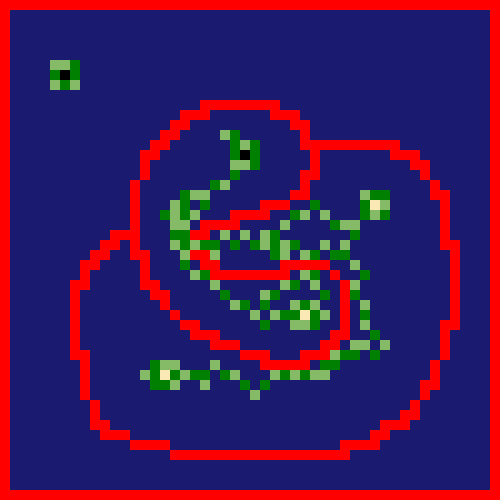
\includegraphics[width=0.5\textwidth]{./images/desarrollo/physarum/Random1.png}}
        \caption{Physarum Polycephalum resolviendo un laberinto de tipo circular.}
        \label{fig:physarumRandom1}    
    \end{figure}
    \begin{figure}[htbp]
        \centerline{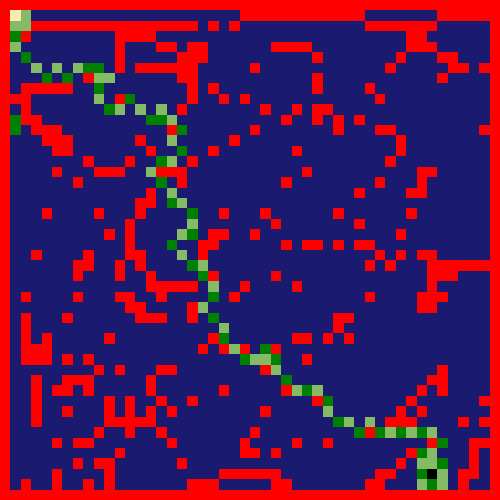
\includegraphics[width=0.5\textwidth]{./images/desarrollo/physarum/Obstaculos1.png}}
        \caption{Physarum Polycephalum resolviendo un laberinto con obst\'aculos.}
        \label{fig:physarumObstacles1}
    \end{figure}
    \vskip 0.5cm
    %P\'arrafo 3
    Gracias a la resoluci\'on de la fuga en las esquinas por nuestro algoritmo, es posible generar mapeos m\'as diversos 
        de cuevas y catacumbas. Este enfoque mejora significativamente nuestra comprensi\'on 
        de la topograf\'ia del \'area explorada. Adem\'as, la diversidad en el mapeo facilita la identificaci\'on 
        del n\'umero y variedad de caminos disponibles, lo que se ha implementado mediante un algoritmo de mapeo de im\'agenes que 
        ayuda en la representaci\'on gr\'afica de dicha topograf\'ia, como se muestra en la Fig \ref{fig:CaveSystemPhysarum}.
    \vskip 0.5cm
        \begin{figure}[htbp]
            \centerline{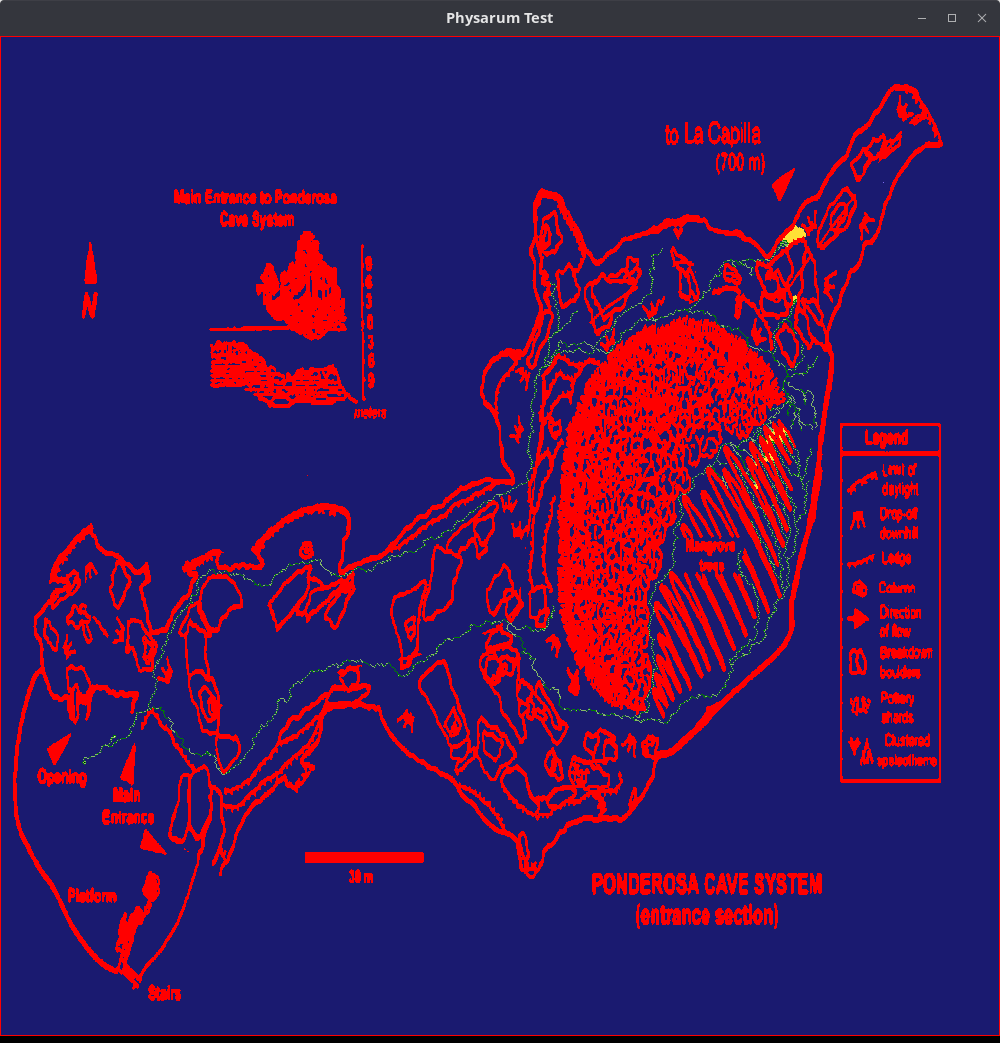
\includegraphics[width=0.40\textwidth]{./images/desarrollo/physarum/CaveSystemPhysarum.png}}
            \caption{Mapeo del sistema de cuevas usando Physarum Polycephalum.}
            \label{fig:CaveSystemPhysarum}
        \end{figure}
        \vskip 0.2cm
        Tambi\'en el algoritmo ha sido probado en un entorno real, donde ha sido capaz de generar 
            rutas \'optimas en la Catacumba de Par\'is, como se muestra en la Fig \ref{fig:Catacomb}. El espacio
            explorado por el algoritmo es de 1000 x 1000 c\'elulas.
        \vskip 0.2cm
        \begin{figure}[htbp]
            \centerline{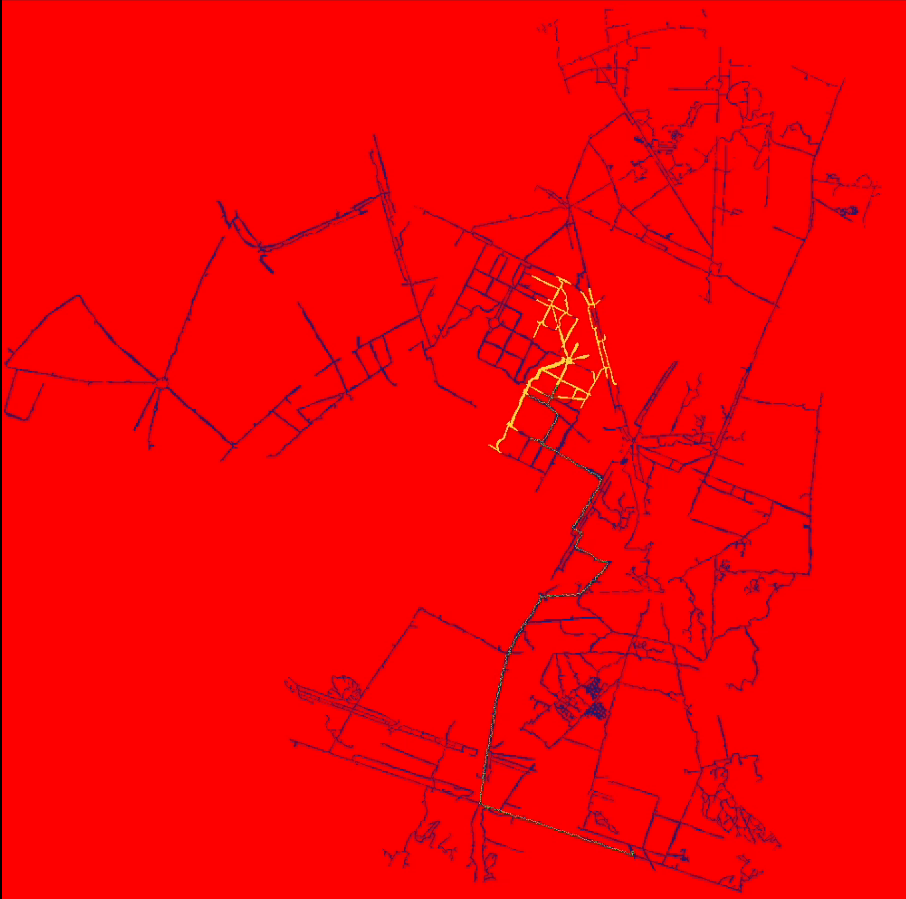
\includegraphics[width=0.40\textwidth]{./images/desarrollo/physarum/CatacoumbParis.png}}
            \caption{Mapeo de la catacumba usando Physarum Polycephalum, utiliza 5264 pasos para obtener la ruta.}
            \label{fig:Catacomb}
        \end{figure}
        %P\'arrafo 4
        Cabe se\~nalar que dado que el algoritmo est\'a bioinspirado, la funci\'on que simula el comportamiento del plasmodio 
            se asigna de manera pseudoaleatoria a un vecino adyacente, con una probabilidad de 1/8. Esta caracter\'istica permite 
            que la expansi\'on del algoritmo tome una forma circular en lugar de una expansi\'on cuadrada o lineal. Sin embargo, al 
            modificar la funci\'on de probabilidad, es posible lograr una expansi\'on m\'as irregular en lugar de simplemente circular.
        \clearpage
        En cuanto la implementaci\'on del algoritmo, se ha utilizado el lenguaje de programaci\'on C++ y la librer\'ia OpenCV para la 
            obtenci\'on de im\'agenes. La parte de las esquinas que mencionamos con anterioridad se implement\'o de la siguiente manera: 
        \begin{lstlisting}[language={C++}, caption={Implementaci\'on del problema de las esquinas}, label={Script}]
            std::vector<int> Physarum::isOnCorner(std::vector<int> neighboursData) {
            std::vector<int> corners;
                if (neighboursData[0] == 2 && neighboursData[2] == 2) {
                    corners.push_back(1);
                }
                if (neighboursData[0] == 2 && neighboursData[6] == 2) {
                    corners.push_back(7);
                }
                if (neighboursData[6] == 2 && neighboursData[4] == 2) {
                    corners.push_back(5);
                }
                if (neighboursData[2] == 2 && neighboursData[4] == 2) {
                    corners.push_back(3);
                }
            return corners;
            }
        \end{lstlisting}
        %P\'arrafo 5
        En el c\'odigo \ref{Script}, se muestra la implementaci\'on de la funci\'on que detecta si el agente se encuentra en una esquina. 
            La funci\'on recibe un vector de enteros que representa los estados de los vecinos adyacentes. Si dos esquinas adyacentes 
            presentan repelentes, la funci\'on devuelve un vector con las esquinas en las que se encuentra el agente. 
            En caso contrario, la funci\'on devuelve un vector vac\'io.
        \vskip 0.5cm
        %P\'arrafo 6
        Por ello podemos decir que el algoritmo propuesto es capaz de resolver laberintos de manera eficiente, 
            generando rutas \'optimas en entornos complejos y desconocidos. Adem\'as, el algoritmo es capaz de 
            adaptarse a diferentes topograf\'ias, lo que lo convierte en una herramienta vers\'atil para la exploraci\'on 
            de entornos desconocidos y nos es de ayuda en el monitoreo de poblaciones y sistemas relacionados.
        \vskip 0.5cm
        
% subsection subsection name (end)
    \subsection{Robot Propuesto} % (fold)
\label{sub:Robot Propuesto}
    Para construir el robot, se emplear\'an diversos materiales, cada uno con una funci\'on espec\'ifica para asegurar 
        la operatividad y eficiencia del dispositivo. A continuaci\'on, se detallan los materiales y sus descripciones.
    \vskip 0.5cm
    El controlador para el motor paso a paso, Nema 23, ser\'a fundamental para manejar el movimiento del robot. 
        Este componente incluye un controlador de motor a pasos que se utilizar\'a en cuatro unidades para garantizar 
        un control preciso de los motores. Los motores a pasos Nema 23 son conocidos por su precisi\'on y confiabilidad, 
        y en este caso, se utilizar\'an cuatro unidades, cada una con una placa frontal de 2.15 x 2.15 pulgadas (57 x 57 mm).
    \vskip 0.5cm
    Para la estructura del robot, se utilizar\'a una l\'amina de aluminio de calibre 14 (1.9 mm) con dimensiones de 20 cm x 40 cm, 
        que proporcionar\'a una base s\'olida y resistente. Adem\'as, se emplear\'an perfiles de aluminio 2040, espec\'ificamente de 20 x 
        40 mm y 500 mm de longitud, en dos unidades, para construir el marco del robot. Tambi\'en se utilizar\'an barras redondas 
        s\'olidas de aluminio de 2 1/2" x 12", en cuatro unidades, para reforzar la estructura y proporcionar soporte adicional.
    \vskip 0.5cm
    La movilidad del robot ser\'a posible gracias a las ruedas omnidireccionales de 6 pulgadas (152 mm) con rodamientos de silicona 
        y cubos de aleaci\'on de aluminio, en cuatro unidades. Estas ruedas permitir\'an un movimiento fluido en m\'ultiples direcciones. 
        Adem\'as, se utilizar\'an diversos tornillos y tuercas, con un paquete de 60 unidades, para ensamblar todas las partes del 
        robot de manera segura.
    \vskip 0.5cm
    Para la energ\'ia, se utilizar\'an bater\'ias de litio de 12V y 20000mAh, recargables, que proporcionar\'an la energ\'ia necesaria 
        para la operaci\'on del robot. Se utilizar\'an dos de estas bater\'ias. Un cargador de bater\'ias de 14V y 20A, espec\'ifico 
        para bater\'ias de litio de 12V, ser\'a empleado para mantener las bater\'ias recargadas y operativas.
    \vskip 0.5cm
    La electr\'onica del robot incluir\'a una Raspberry Pi 4 B, que actuar\'a como el cerebro del dispositivo, gestionando 
        las operaciones y los datos recibidos. Un sensor de distancia Detecci\'on y Rango de Luz (Light Detection and Ranging, LiDAR), modelo DTOF STL27L, permitir\'a al 
        robot detectar obst\'aculos y medir distancias con precisi\'on, utilizando un l\'aser LiDAR 360\degree con bus UART 
        y un rango de 895 - 915 NM (tipo 905).
    \vskip 0.5cm
    Para la visi\'on, se emplear\'a una c\'amara de visi\'on nocturna de luz infrarroja de 5MP, con un \'angulo de visi\'on de 
        130-220 grados, espec\'ifica para la Raspberry Pi 4B. Tambi\'en se incluir\'a un convertidor auto Boost Buck de CD-CD, 
        de 5A y rango de 5V-30V, que ayudar\'a a gestionar las diferentes necesidades de voltaje de los componentes 
        electr\'onicos del robot.
    \vskip 0.5cm
    Finalmente, se utilizar\'a una l\'amina de acr\'ilico transparente de 6 mm, con dimensiones de 60 x 120 cm, 
        para crear cubiertas protectoras y otras partes visibles del robot. Este material es ideal por su 
        durabilidad y resistencia a impactos.
    \vskip 0.5cm
    Estos componentes, cuidadosamente seleccionados, se ensamblar\'an para crear un robot funcional, 
        robusto y vers\'atil, capaz de realizar diversas tareas con eficiencia y precisi\'on.
    \vskip 0.5cm
    Ahora claro ense\~namos lo que ser\'ia la primera versi\'on del sistema de control del robot propuesto.
    \subsubsection{Desarrollo Inicial del Sistema del control del Robot}
\label{sub:Desarrollo Inicial del Sistema del control del Robot}
    En esta subsecci\'on nos centramos en desarrollar el c\'odigo inicial para poder controlar el robot, el cual se puede ver en el Listing \ref{PrimeraVersionCodigoRobot}.
    \vskip 0.5cm
    \begin{lstlisting}[language={C++}, caption={Primera versi\'on del c\'odigo del sistema de control del robot}, label={PrimeraVersionCodigoRobot}]
        #include "CYdLidar.h"
        #include <SFML/Graphics.hpp>
        #include <opencv2/opencv.hpp>
        #include <iostream>
        #include <cstdlib>
        #include <cstdio>
        #include <pigpio.h>
        #include <string>
        #include <map>
        #include <vector>
        #include <atomic>
        #include <thread>
        #include <random>
        
        using namespace std;
        using namespace ydlidar;
        
        // Pines y configuraci\'on para los motores
        const int PWM_PINS[] = {13, 19, 18, 12};  // Pines PWM para los motores
        const int DIR_PINS[] = {5, 6, 23, 24};    // Pines de direcci\'on para los motores
        int frequency = 400; // Frecuencia inicial
        
        std::atomic<bool> is_running(true);
        std::atomic<bool> is_manual_mode(true);
        
        void setMotorSpeed(int motor, int frequency) {
            if (motor >= 0 && motor < 4) {
                gpioSetPWMfrequency(PWM_PINS[motor], frequency);
            }
        }
        
        void setMotorDirection(int motor, int direction) {
            if (motor >= 0 && motor < 4) {
                gpioWrite(DIR_PINS[motor], direction);
            }
        }
        
        void stopMotors() {
            for (int i = 0; i < 4; ++i) {
                gpioPWM(PWM_PINS[i], 0);
            }
        }
        
        void moveForward() {
            for (int i = 0; i < 4; ++i) {
                gpioPWM(PWM_PINS[i], 128);  // Establecer ciclo de trabajo al 50%
            }
            setMotorDirection(0, 0); // Motor 1
            setMotorDirection(2, 0); // Motor 3
            setMotorDirection(1, 1); // Motor 2
            setMotorDirection(3, 1); // Motor 4
        }
        
        void moveBackward() {
            for (int i = 0; i < 4; ++i) {
                gpioPWM(PWM_PINS[i], 128);  // Establecer ciclo de trabajo al 50%
            }
            setMotorDirection(0, 1); // Motor 1
            setMotorDirection(2, 1); // Motor 3
            setMotorDirection(1, 0); // Motor 2
            setMotorDirection(3, 0); // Motor 4
        }
        
        void turnLeft() {
            for (int i = 0; i < 4; ++i) {
                gpioPWM(PWM_PINS[i], 128);  // Establecer ciclo de trabajo al 50%
            }
            setMotorDirection(0, 1); // Motor 1
            setMotorDirection(2, 1); // Motor 3
            setMotorDirection(1, 1); // Motor 2
            setMotorDirection(3, 1); // Motor 4
        }
        
        void turnRight() {
            for (int i = 0; i < 4; ++i) {
                gpioPWM(PWM_PINS[i], 128);  // Establecer ciclo de trabajo al 50%
            }
            setMotorDirection(0, 0); // Motor 1
            setMotorDirection(2, 0); // Motor 3
            setMotorDirection(1, 0); // Motor 2
            setMotorDirection(3, 0); // Motor 4
        }
        
        void increaseSpeed() {
            if (frequency < 1600) {
                frequency += 100;
                if (frequency > 1600) frequency = 1600;
                for (int i = 0; i < 4; ++i) {
                    setMotorSpeed(i, frequency);
                }
            }
        }
        
        void decreaseSpeed() {
            if (frequency > 400) {
                frequency -= 100;
                if (frequency < 400) frequency = 400;
                for (int i = 0; i < 4; ++i) {
                    setMotorSpeed(i, frequency);
                }
            }
        }
        
        sf::Color getPointColor(float distance, float maxRange) {
            float ratio = distance / maxRange;
            return sf::Color(255 * (1 - ratio), 255 * ratio, 0); // Color de rojo a verde
        }
        
        void randomMovement(CYdLidar &laser) {
            std::random_device rd;
            std::mt19937 gen(rd());
            std::discrete_distribution<> dist({1, 10, 10, 70}); // Distribuci\'on para la probabilidad de movimiento
        
            while (is_running) {
                if (!is_manual_mode) {
                    LaserScan scan;
                    if (laser.doProcessSimple(scan)) {
                        bool obstacle_detected = false;
                        for (const auto &point : scan.points) {
                            if (point.range < 0.35) {  // Detecta un obst\'aculo a 35 cm
                                obstacle_detected = true;
                                break;
                            }
                        }
        
                        if (obstacle_detected) {
                            // Si detecta un obst\'aculo, retrocede por 4 segundos
                            moveBackward();
                            std::this_thread::sleep_for(std::chrono::seconds(4));
                            stopMotors();
        
                            // Luego gira aleatoriamente a la izquierda o derecha
                            int turn = dist(gen) % 2;
                            if (turn == 0) {
                                turnLeft();
                            } else {
                                turnRight();
                            }
                            std::this_thread::sleep_for(std::chrono::seconds(2));
                            stopMotors();
                        } else {
                            // Si no hay obst\'aculo, elige un movimiento aleatorio
                            int move = dist(gen);
                            switch (move) {
                                case 0: moveBackward(); break;
                                case 1: turnRight(); break;
                                case 2: turnLeft(); break;
                                case 3: moveForward(); break;
                            }
                        }
                    }
                    std::this_thread::sleep_for(std::chrono::milliseconds(500));
                    stopMotors();
                }
                std::this_thread::sleep_for(std::chrono::milliseconds(100));
            }
        }
        
        int main() {
            // Inicializar pigpio
            if (gpioInitialise() < 0) {
                std::cerr << "Error: No se pudo inicializar pigpio." << std::endl;
                return -1;
            }
        
            // Configurar pines de direcci\'on como salida
            for (int i = 0; i < 4; ++i) {
                gpioSetMode(DIR_PINS[i], PI_OUTPUT);
                gpioSetMode(PWM_PINS[i], PI_OUTPUT);
                setMotorSpeed(i, frequency);  // Inicializar PWM con frecuencia inicial
            }
        
            // Aseg\'urate de establecer XDG_RUNTIME_DIR
            if (getenv("XDG_RUNTIME_DIR") == nullptr) {
                setenv("XDG_RUNTIME_DIR", "/tmp/runtime-$(id -u)", 1);
            }
        
            // Ejecuta libcamera-vid en un proceso separado y captura la salida en YUV, sin previsualizaci\'on
            FILE* pipe = popen("libcamera-vid -t 0 --codec yuv420 --nopreview -o -", "r");
            if (!pipe) {
                std::cerr << "Error: No se pudo ejecutar libcamera-vid." << std::endl;
                return -1;
            }
        
            // Configura la ventana SFML
            sf::RenderWindow window(sf::VideoMode(1280, 720), "Camera Visualization with LiDAR");
            sf::Texture cameraTexture;
            sf::Sprite cameraSprite;
        
            // Buffer para leer los datos de video
            const int width = 640;
            const int height = 480;
            std::vector<uint8_t> buffer(width * height * 3 / 2); // Ajusta el tama\~no del buffer para YUV420
        
            cv::Mat yuvImage(height + height / 2, width, CV_8UC1, buffer.data());
            cv::Mat rgbImage(height, width, CV_8UC3);
        
            std::string port;
            ydlidar::os_init();
        
            // Obtener los puertos disponibles de LiDAR
            std::map<std::string, std::string> ports = ydlidar::lidarPortList();
            if (ports.size() > 1) {
                auto it = ports.begin();
                std::advance(it, 1); // Selecciona el segundo puerto disponible
                port = it->second;
            } else if (ports.size() == 1) {
                port = ports.begin()->second;
            } else {
                std::cerr << "No se detect\'o ning\'un LiDAR. Verifica la conexi\'on." << std::endl;
                return -1;
            }
        
            // Configuraci\'on del LiDAR
            int baudrate = 115200;
            std::cout << "Baudrate: " << baudrate << std::endl;
        
            CYdLidar laser;
            laser.setlidaropt(LidarPropSerialPort, port.c_str(), port.size());
            laser.setlidaropt(LidarPropSerialBaudrate, &baudrate, sizeof(int));
        
            bool isSingleChannel = true;
            laser.setlidaropt(LidarPropSingleChannel, &isSingleChannel, sizeof(bool));
        
            float max_range = 8.0f;
            float min_range = 0.1f;
            float max_angle = 180.0f;
            float min_angle = -180.0f;
            float frequency = 8.0f;
        
            laser.setlidaropt(LidarPropMaxRange, &max_range, sizeof(float));
            laser.setlidaropt(LidarPropMinRange, &min_range, sizeof(float));
            laser.setlidaropt(LidarPropMaxAngle, &max_angle, sizeof(float));
            laser.setlidaropt(LidarPropMinAngle, &min_angle, sizeof(float));
            laser.setlidaropt(LidarPropScanFrequency, &frequency, sizeof(float));
        
            // Inicializar LiDAR
            if (!laser.initialize()) {
                std::cerr << "Error al inicializar el LiDAR." << std::endl;
                return -1;
            }
        
            // Iniciar el escaneo
            if (!laser.turnOn()) {
                std::cerr << "Error al encender el LiDAR." << std::endl;
                return -1;
            }
        
            // Thread para movimiento aleatorio
            std::thread randomMoveThread(randomMovement, std::ref(laser));
        
            while (window.isOpen()) {
                sf::Event event;
                while (window.pollEvent(event)) {
                    if (event.type == sf::Event::Closed)
                        window.close();
        
                    if (event.type == sf::Event::KeyPressed) {
                        switch (event.key.code) {
                            case sf::Keyboard::W:
                                is_manual_mode = true;
                                moveForward();
                                break;
                            case sf::Keyboard::S:
                                is_manual_mode = true;
                                moveBackward();
                                break;
                            case sf::Keyboard::A:
                                is_manual_mode = true;
                                turnLeft();
                                break;
                            case sf::Keyboard::D:
                                is_manual_mode = true;
                                turnRight();
                                break;
                            case sf::Keyboard::Add:
                                is_manual_mode = true;
                                increaseSpeed();
                                break;
                            case sf::Keyboard::Subtract:
                                is_manual_mode = true;
                                decreaseSpeed();
                                break;
                            case sf::Keyboard::Space:
                                is_manual_mode = true;
                                stopMotors();
                                break;
                            case sf::Keyboard::K:
                                is_manual_mode = false;
                                break;
                            case sf::Keyboard::M:
                                is_manual_mode = true;
                                break;
                            default:
                                break;
                        }
                    }
                }
        
                // Leer los datos del video desde la tuber\'ia
                size_t bytesRead = fread(buffer.data(), 1, buffer.size(), pipe);
                if (bytesRead != buffer.size()) {
                    std::cerr << "Error: No se pudo leer suficientes datos de video." << std::endl;
                    continue;
                }
        
                // Convertir YUV420 a RGB
                cv::cvtColor(yuvImage, rgbImage, cv::COLOR_YUV2RGB_I420);
        
                // Convertir a RGBA a\~nadiendo un canal alfa
                cv::Mat frame_rgba;
                cv::cvtColor(rgbImage, frame_rgba, cv::COLOR_RGB2RGBA);
        
                // Actualizar la textura de la c\'amara con los datos del frame
                if (!cameraTexture.create(frame_rgba.cols, frame_rgba.rows)) {
                    std::cerr << "Error: No se pudo crear la textura." << std::endl;
                    continue;
                }
                cameraTexture.update(frame_rgba.ptr());
        
                cameraSprite.setTexture(cameraTexture);
                cameraSprite.setScale(
                    window.getSize().x / static_cast<float>(cameraTexture.getSize().x),
                    window.getSize().y / static_cast<float>(cameraTexture.getSize().y)
                );
        
                window.clear();
                window.draw(cameraSprite);
        
                // Crear un minimapa para el LiDAR
                sf::RectangleShape minimap(sf::Vector2f(200, 200));
                minimap.setFillColor(sf::Color(200, 200, 200, 150)); // Fondo semitransparente
                minimap.setPosition(10, 10); // Esquina superior izquierda
        
                window.draw(minimap);
        
                // Dibujar el centro del LiDAR (color azul)
                sf::CircleShape lidarCenter(5); // Radio del c\'irculo del LiDAR
                lidarCenter.setFillColor(sf::Color::Blue);
                lidarCenter.setPosition(105, 105); // Posici\'on del centro en el minimapa
        
                window.draw(lidarCenter);
        
                // Dibujar la l\'inea hacia el norte
                sf::Vertex line[] =
                {
                    sf::Vertex(sf::Vector2f(110, 110), sf::Color::Black),
                    sf::Vertex(sf::Vector2f(110, 60), sf::Color::Black) // L\'inea hacia arriba (norte)
                };
        
                window.draw(line, 2, sf::Lines);
        
                LaserScan scan;
                if (laser.doProcessSimple(scan)) {
                    for (const auto& point : scan.points) {
                        // Convertir coordenadas polares a cartesianas
                        float x = point.range * cos(point.angle);
                        float y = point.range * sin(point.angle);
        
                        // Ajustar los puntos al minimapa
                        float scale = 25.0f;
                        float adjustedX = 110 + x * scale;
                        float adjustedY = 110 - y * scale; // Invertir Y para coordinar con la pantalla
        
                        // Dibujar los puntos en el minimapa, excluyendo el centro (0,0)
                        if (point.range > 0.05) {
                            sf::CircleShape lidarPoint(2);
                            lidarPoint.setPosition(adjustedX, adjustedY);
                            lidarPoint.setFillColor(getPointColor(point.range, max_range));
        
                            window.draw(lidarPoint);
                        }
                    }
                } else {
                    std::cerr << "No se pudieron obtener los datos del LiDAR." << std::endl;
                }
        
                window.display();
            }
        
            // Detener el escaneo del LiDAR
            laser.turnOff();
            laser.disconnecting();
        
            // Cierra la tuber\'ia, detiene los motores y apaga el robot
            pclose(pipe);
            stopMotors();
            gpioTerminate();
        
            is_running = false;
            randomMoveThread.join();
        
            return 0;
        }
    \end{lstlisting}

    En el Listing \ref{PrimeraVersionCodigoRobot} se inicializan los motores y se establecen las funciones para controlar el movimiento del robot. 
        Adem\'as, se configura el LiDAR y se inicia el escaneo. El robot se mueve aleatoriamente y evita obst\'aculos 
        detectados por el LiDAR. La c\'amara muestra la vista del robot y el minimapa muestra los puntos detectados por 
        el LiDAR. El usuario puede controlar manualmente el robot con las teclas W, A, S y D para moverse hacia adelante, 
        izquierda, atr\'as y derecha, respectivamente. Las teclas V y B aumentan y disminuyen la velocidad del robot, 
        respectivamente. La tecla Espacio detiene el robot. La tecla K activa el modo autom\'atico y la tecla M activa 
        el modo manual. El robot se mueve aleatoriamente y evita obst\'aculos detectados por el LiDAR. El c\'odigo se ejecuta 
        en un bucle hasta que se cierra la ventana de la c\'amara. Al final, se detiene el escaneo del LiDAR y se apaga el robot.
    
    \subsubsection{Ajustes de c\'odigo en funci\'on de pruebas unitarias y de aceptaci\'on 1}
\label{subsub:Ajustes de c\'odigo en funci\'on de pruebas unitarias y de aceptaci\'on}
%Funciono bien, menos el modo aleatorio, que se movia de mala manera por
% como le ordenaba moverse, por lo que se ajusto el c\'odigo para que se
% moviera de manera m\'as eficiente.
%parrafo 1 
    El c\'odigo del robot funcion\'o correctamente en las pruebas unitarias y de aceptaci\'on, 
    con la excepci\'on del modo aleatorio, que present\'o problemas de movimiento.
    %parrafo 2
    El robot se mov\'ia de manera ineficiente en el modo aleatorio, debido a la forma en 
    que se le ordenaba moverse y que en 0,0 detectaba obstaculos donde no los habia, en otras palabras daba 
    falsos positivos. Por lo tanto, se realizaron ajustes en el c\'odigo para 
    mejorar su desempe\~no y eficiencia, los cuales se pueder ver en el Listing \ref{PrimerAjuste}.
% subsection Ajustes de c\'odigo en funci\'on de pruebas unitarias y de aceptaci\'on (end)
%listnig de la seccion
\begin{lstlisting}[language={C++}, caption={Primer ajuste de c\'odigo}, label={PrimerAjuste}]
    #include "CYdLidar.h"
    #include <SFML/Graphics.hpp>
    #include <opencv2/opencv.hpp>
    #include <iostream>
    #include <cstdlib>
    #include <cstdio>
    #include <pigpio.h>
    #include <string>
    #include <map>
    #include <vector>
    #include <atomic>
    #include <thread>
    #include <random>
    #include <sys/socket.h>
    #include <sys/un.h>
    #include <unistd.h>
    #include <cstring>
    #include <pthread.h>
    #include <vector>
    #include <mutex>
    
    using namespace std;
    using namespace ydlidar;
    
    // Pines y configuracin para los motores
    const int PWM_PINS[] = {13, 19, 18, 12};  // Pines PWM para los motores
    const int DIR_PINS[] = {5, 6, 23, 24};    // Pines de direccin para los motores
    int frequency = 400; // Frecuencia inicial
    
    std::atomic<bool> is_running(true);
    std::atomic<bool> is_manual_mode(true);
    
    void setMotorSpeed(int motor, int frequency) {
        if (motor >= 0 && motor < 4) {
            gpioSetPWMfrequency(PWM_PINS[motor], frequency);
        }
    }
    
    void setMotorDirection(int motor, int direction) {
        if (motor >= 0 && motor < 4) {
            gpioWrite(DIR_PINS[motor], direction);
        }
    }
    
    void stopMotors() {
        for (int i = 0; i < 4; ++i) {
            gpioPWM(PWM_PINS[i], 0);
        }
    }
    
    void moveForward() {
        for (int i = 0; i < 4; ++i) {
            gpioPWM(PWM_PINS[i], 128);  // Establecer ciclo de trabajo al 50%
        }
        setMotorDirection(0, 0); // Motor 1
        setMotorDirection(2, 0); // Motor 3
        setMotorDirection(1, 1); // Motor 2
        setMotorDirection(3, 1); // Motor 4
    }
    
    void moveBackward() {
        for (int i = 0; i < 4; ++i) {
            gpioPWM(PWM_PINS[i], 128);  // Establecer ciclo de trabajo al 50%
        }
        setMotorDirection(0, 1); // Motor 1
        setMotorDirection(2, 1); // Motor 3
        setMotorDirection(1, 0); // Motor 2
        setMotorDirection(3, 0); // Motor 4
    }
    
    void turnLeft() {
        for (int i = 0; i < 4; ++i) {
            gpioPWM(PWM_PINS[i], 128);  // Establecer ciclo de trabajo al 50%
        }
        setMotorDirection(0, 1); // Motor 1
        setMotorDirection(2, 1); // Motor 3
        setMotorDirection(1, 1); // Motor 2
        setMotorDirection(3, 1); // Motor 4
    }
    
    void turnRight() {
        for (int i = 0; i < 4; ++i) {
            gpioPWM(PWM_PINS[i], 128);  // Establecer ciclo de trabajo al 50%
        }
        setMotorDirection(0, 0); // Motor 1
        setMotorDirection(2, 0); // Motor 3
        setMotorDirection(1, 0); // Motor 2
        setMotorDirection(3, 0); // Motor 4
    }
    
    void increaseSpeed() {
        if (frequency < 2000) {
            frequency += 100;
            if (frequency > 2000) frequency = 2000;
            for (int i = 0; i < 4; ++i) {
                setMotorSpeed(i, frequency);
            }
        }
    }
    
    void decreaseSpeed() {
        if (frequency > 400) {
            frequency -= 100;
            if (frequency < 400) frequency = 400;
            for (int i = 0; i < 4; ++i) {
                setMotorSpeed(i, frequency);
            }
        }
    }
    
    
    sf::Color getPointColor(float distance, float maxRange) {
        float ratio = distance / maxRange;
        return sf::Color(255 * (1 - ratio), 255 * ratio, 0); // Color de rojo a verde
    }
    
    int contadorObstaculoTotal = 0;
    int obstaculoHola = 0;
    int obsRelativo = 0;
    void randomMovement(CYdLidar &laser) {
        std::random_device rd;
        std::mt19937 gen(rd());
        std::discrete_distribution<> dist({1, 0, 10, 70}); // Distribucin para la probabilidad de movimiento
    
        const float FRONT_MIN_ANGLE = -10.0f * (M_PI / 180.0f); // -15 grados en radaianes
        const float FRONT_MAX_ANGLE = 10.0f * (M_PI / 180.0f);  // 15 grados en radianes
        const float DETECTION_RADIUS = 0.25f; // 35 cm
    
        std::vector<float> previousScanPoints;
    
        while (is_running) {
            if (!is_manual_mode) {
                LaserScan scan;
                if (laser.doProcessSimple(scan)) {
                    bool obstacle_detected = false;
                    std::vector<float> currentScanPoints;
                    
                    for (const auto &point : scan.points) {
                        // Convertir el ngulo del punto al ngulo relativo al "sur" del robot
                        float adjusted_angle = point.angle + M_PI;
                        //std::cout << "Er " << point.range << std::endl;
                        // Verificar si el punto est dentro del rango frontal de 30
                        if (point.range > 0 &&point.range < 0.40 && abs(point.angle) < adjusted_angle) {
                            obstacle_detected = true;
                            currentScanPoints.push_back(point.range);
                            std::cout << "Obstacle distance: " << (float)point.range  << " Y en el angulo  "<<point.angle << std::endl;
                            break;
                        }
                    }
                    
                    if (obstacle_detected) {
                        // Si detecta un obstculo, retrocede por 4 segundos
                        contadorObstaculoTotal++;
                        std::cout << "Obs: " << contadorObstaculoTotal << std::endl;
                        //obsRelativo++;
                        stopMotors();
                        //Luego gira aleatoriamente a la izquierda o derecha
                        int turn = dist(gen) % 2;
                        if (turn == 0) {
                            turnLeft();
                            std::this_thread::sleep_for(std::chrono::seconds(5));
                        } else {
                            turnRight();
                            std::this_thread::sleep_for(std::chrono::seconds(5));
                        }
                        std::this_thread::sleep_for(std::chrono::seconds(2));
                        stopMotors();
                        
                        if(!previousScanPoints.empty() && previousScanPoints.size() == currentScanPoints.size()){
                                bool mismoObs = true;
                                for(size_t i = 0; i < currentScanPoints.size(); ++i){
                                    if(fabs(currentScanPoints[i] - previousScanPoints[i]) > 0.05){
                                            mismoObs = false;
                                            break;
                                    }
                                }
                                if(mismoObs){
                                    obsRelativo++;
                                }else{
                                    obsRelativo = 0;
                                }
                        }
                        
                        previousScanPoints = currentScanPoints;
                        
                        if((obsRelativo > 3)){
                            //obsRelativo = 0;
                            moveBackward();
                            std::this_thread::sleep_for(std::chrono::seconds(3));
                            stopMotors();
                            int turn = dist(gen) % 2;
                            if (turn == 0) {
                                turnLeft();
                                std::this_thread::sleep_for(std::chrono::seconds(5));
                            } else {
                                turnRight();
                                std::this_thread::sleep_for(std::chrono::seconds(5));
                            }
                                std::this_thread::sleep_for(std::chrono::seconds(2));
                                stopMotors();
                        }
                    } else {
                        moveForward();
                        // Si no hay obstculo, elige un movimiento aleatorio
                        //
                        //int move = dist(gen);
                        //switch (move) {
                          //  case 0: moveBackward(); break;
                          //  case 1: turnRight(); break;
                          //  case 2: turnLeft(); break;
                          //  case 3: moveForward(); break;
                        //}
                    }
                }
                
                std::this_thread::sleep_for(std::chrono::milliseconds(500));
                //stopMotors();
            }
            std::this_thread::sleep_for(std::chrono::milliseconds(100));
        }
    }
    
    int main() {
        // Inicializar pigpio
        if (gpioInitialise() < 0) {
            std::cerr << "Error: No se pudo inicializar pigpio." << std::endl;
            return -1;
        }
    
        // Configurar pines de direccin como salida
        for (int i = 0; i < 4; ++i) {
            gpioSetMode(DIR_PINS[i], PI_OUTPUT);
            gpioSetMode(PWM_PINS[i], PI_OUTPUT);
            setMotorSpeed(i, frequency);  // Inicializar PWM con frecuencia inicial
        }
    
        // Asegrate de establecer XDG_RUNTIME_DIR
        if (getenv("XDG_RUNTIME_DIR") == nullptr) {
            setenv("XDG_RUNTIME_DIR", "/tmp/runtime-$(id -u)", 1);
        }
    
        // Ejecuta libcamera-vid en un proceso separado y captura la salida en YUV, sin previsualizacn
        FILE* pipe = popen("libcamera-vid -t 0 --codec yuv420 --nopreview -o -", "r");
        if (!pipe) {
            std::cerr << "Error: No se pudo ejecutar libcamera-vid." << std::endl;
            return -1;
        }
    
        // Configura la ventana SFML
        sf::RenderWindow window(sf::VideoMode(1280, 720), "Camera Visualization with LiDAR");
        sf::Texture cameraTexture;
        sf::Sprite cameraSprite;
    
        // Buffer para leer los datos de video
        const int width = 640;
        const int height = 480;
        std::vector<uint8_t> buffer(width * height * 3 / 2); // Ajusta el tamao del buffer para YUV420
    
        cv::Mat yuvImage(height + height / 2, width, CV_8UC1, buffer.data());
        cv::Mat rgbImage(height, width, CV_8UC3);
    
        std::string port;
        ydlidar::os_init();
    
        // Obtener los puertos disponibles de LiDAR
        std::map<std::string, std::string> ports = ydlidar::lidarPortList();
        if (ports.size() > 1) {
            auto it = ports.begin();
            std::advance(it, 1); // Selecciona el segundo puerto disponible
            port = it->second;
        } else if (ports.size() == 1) {
            port = ports.begin()->second;
        } else {
            std::cerr << "No se detect ningn LiDAR. Verifica la conexin." << std::endl;
            return -1;
        }
    
        // Configuracin del LiDAR
        int baudrate = 115200;
        std::cout << "Baudrate: " << baudrate << std::endl;
    
        CYdLidar laser;
        laser.setlidaropt(LidarPropSerialPort, port.c_str(), port.size());
        laser.setlidaropt(LidarPropSerialBaudrate, &baudrate, sizeof(int));
    
        bool isSingleChannel = true;
        laser.setlidaropt(LidarPropSingleChannel, &isSingleChannel, sizeof(bool));
    
        float max_range = 8.0f;
        float min_range = 0.1f;
        float max_angle = 180.0f;
        float min_angle = -180.0f;
        float frequency = 8.0f;
    
        laser.setlidaropt(LidarPropMaxRange, &max_range, sizeof(float));
        laser.setlidaropt(LidarPropMinRange, &min_range, sizeof(float));
        laser.setlidaropt(LidarPropMaxAngle, &max_angle, sizeof(float));
        laser.setlidaropt(LidarPropMinAngle, &min_angle, sizeof(float));
        laser.setlidaropt(LidarPropScanFrequency, &frequency, sizeof(float));
    
        // Inicializar LiDAR
        if (!laser.initialize()) {
            std::cerr << "Error al inicializar el LiDAR." << std::endl;
            return -1;
        }
    
        // Iniciar el escaneo
        if (!laser.turnOn()) {
            std::cerr << "Error al encender el LiDAR." << std::endl;
            return -1;
        }
    
        // Thread para movimiento aleatorio
        std::thread randomMoveThread(randomMovement, std::ref(laser));
    
        while (window.isOpen()) {
            sf::Event event;
            while (window.pollEvent(event)) {
                if (event.type == sf::Event::Closed)
                    window.close();
    
                if (event.type == sf::Event::KeyPressed) {
                    switch (event.key.code) {
                        case sf::Keyboard::W:
                            is_manual_mode = true;
                            moveForward();
                            break;
                        case sf::Keyboard::S:
                            is_manual_mode = true;
                            moveBackward();
                            break;
                        case sf::Keyboard::A:
                            is_manual_mode = true;
                            turnLeft();
                            break;
                        case sf::Keyboard::D:
                            is_manual_mode = true;
                            turnRight();
                            break;
                        case sf::Keyboard::V:
                            is_manual_mode = true;
                            increaseSpeed();
                            break;
                        case sf::Keyboard::B:
                            is_manual_mode = true;
                            decreaseSpeed();
                            break;
                        case sf::Keyboard::Space:
                            is_manual_mode = true;
                            stopMotors();
                            break;
                        case sf::Keyboard::K:
                            is_manual_mode = false;
                            break;
                        case sf::Keyboard::M:
                            is_manual_mode = true;
                            break;
                        default:
                            break;
                    }
                }
            }
    
            // Leer los datos del video desde la tubera
            size_t bytesRead = fread(buffer.data(), 1, buffer.size(), pipe);
            if (bytesRead != buffer.size()) {
                std::cerr << "Error: No se pudo leer suficientes datos de video." << std::endl;
                continue;
            }
    
            // Convertir YUV420 a RGB
            cv::cvtColor(yuvImage, rgbImage, cv::COLOR_YUV2RGB_I420);
    
            // Convertir a RGBA aadiendo un canal alfa
            cv::Mat frame_rgba;
            cv::cvtColor(rgbImage, frame_rgba, cv::COLOR_RGB2RGBA);
    
            // Actualizar la textura de la cmara con los datos del frame
            if (!cameraTexture.create(frame_rgba.cols, frame_rgba.rows)) {
                std::cerr << "Error: No se pudo crear la textura." << std::endl;
                continue;
            }
            cameraTexture.update(frame_rgba.ptr());
    
            cameraSprite.setTexture(cameraTexture);
            cameraSprite.setScale(
                window.getSize().x / static_cast<float>(cameraTexture.getSize().x),
                window.getSize().y / static_cast<float>(cameraTexture.getSize().y)
            );
    
            window.clear();
            window.draw(cameraSprite);
    
            // Crear un minimapa para el LiDAR
            sf::RectangleShape minimap(sf::Vector2f(200, 200));
            minimap.setFillColor(sf::Color(200, 200, 200, 150)); // Fondo semitransparente
            minimap.setPosition(10, 10); // Esquina superior izquierda
    
            window.draw(minimap);
    
            // Dibujar el centro del LiDAR (color azul)
            sf::CircleShape lidarCenter(5); // Radio del crculo del LiDAR
            lidarCenter.setFillColor(sf::Color::Blue);
            lidarCenter.setPosition(105, 105); // Posicin del centro en el minimapa
    
            window.draw(lidarCenter);
    
            // Dibujar la lnea hacia el norte
            sf::Vertex line[] =
            {
                sf::Vertex(sf::Vector2f(110, 110), sf::Color::Black),
                sf::Vertex(sf::Vector2f(110, 160), sf::Color::Black) // Lnea hacia arriba (norte)
            };
    
            window.draw(line, 2, sf::Lines);
    
            LaserScan scan;
            if (laser.doProcessSimple(scan)) {
                for (const auto& point : scan.points) {
                    // Convertir coordenadas polares a cartesianas
                    float x = point.range * cos(point.angle);
                    float y = point.range * sin(point.angle);
    
                    // Ajustar los puntos al minimapa
                    float scale = 25.0f;
                    float adjustedX = 110 + x * scale;
                    float adjustedY = 110 - y * scale; // Invertir Y para coordinar con la pantalla
    
                    // Dibujar los puntos en el minimapa, excluyendo el centro (0,0)
                    if (point.range > 0.05) {
                        sf::CircleShape lidarPoint(2);
                        lidarPoint.setPosition(adjustedX, adjustedY);
                        lidarPoint.setFillColor(getPointColor(point.range, max_range));
    
                        window.draw(lidarPoint);
                    }
                    //std::cout << "An " << point.range <<std :: endl;
                }
            } else {
                std::cerr << "No se pudieron obtener los datos del LiDAR." << std::endl;
            }
    
            window.display();
        }
    
        // Detener el escaneo del LiDAR
        laser.turnOff();
        laser.disconnecting();
    
        // Cierra la tubera, detiene los motores y apaga el robot
        pclose(pipe);
        stopMotors();
        gpioTerminate();
    
        is_running = false;
        randomMoveThread.join();
    
        return 0;
    }
\end{lstlisting}
% section Resultados de las pruebas (end)

    \subsubsection{Ajustes de c\'odigo en funci\'on de pruebas unitarias y de aceptaci\'on 2} % (fold)
\label{ssub:Ajustes de c\'odigo en funci\'on de pruebas unitarias y de aceptaci\'on}
    En este caso se agregaron modificaciones para el mejor funcionamiento del detectar obst\'aculos
    sobre todo los \'angulos de giro y la distancia de detecci\'on de los obst\'aculos. Estas modificaciones
    se realizaron en el c\'odigo principal del robot, el cual se muestra en el Listing \ref{SegundoAjuste}.
    \begin{lstlisting}[language={C++}, caption={Segundo ajuste de c\'odigo}, label={SegundoAjuste}]
        #include "CYdLidar.h"
        #include <SFML/Graphics.hpp>
        #include <opencv2/opencv.hpp>
        #include <iostream>
        #include <cstdlib>
        #include <cstdio>
        #include <pigpio.h>
        #include <string>
        #include <map>
        #include <vector>
        #include <atomic>
        #include <thread>
        #include <random>
        #include <sys/socket.h>
        #include <sys/un.h>
        #include <unistd.h>
        #include <cstring>
        #include <pthread.h>
        #include <vector>
        #include <mutex>
        
        using namespace std;
        using namespace ydlidar;
        
        // Pines y configuracin para los motores
        const int PWM_PINS[] = {13, 19, 18, 12};  // Pines PWM para los motores
        const int DIR_PINS[] = {5, 6, 23, 24};    // Pines de direccin para los motores
        int frequency = 400; // Frecuencia inicial
        
        std::atomic<bool> is_running(true);
        std::atomic<bool> is_manual_mode(true);
        
        void setMotorSpeed(int motor, int frequency) {
            if (motor >= 0 && motor < 4) {
                gpioSetPWMfrequency(PWM_PINS[motor], frequency);
            }
        }
        
        void setMotorDirection(int motor, int direction) {
            if (motor >= 0 && motor < 4) {
                gpioWrite(DIR_PINS[motor], direction);
            }
        }
        
        void stopMotors() {
            for (int i = 0; i < 4; ++i) {
                gpioPWM(PWM_PINS[i], 0);
            }
        }
        
        void moveForward() {
            for (int i = 0; i < 4; ++i) {
                gpioPWM(PWM_PINS[i], 128);  // Establecer ciclo de trabajo al 50%
            }
            setMotorDirection(0, 0); // Motor 1
            setMotorDirection(2, 0); // Motor 3
            setMotorDirection(1, 1); // Motor 2
            setMotorDirection(3, 1); // Motor 4
        }
        
        void moveBackward() {
            for (int i = 0; i < 4; ++i) {
                gpioPWM(PWM_PINS[i], 128);  // Establecer ciclo de trabajo al 50%
            }
            setMotorDirection(0, 1); // Motor 1
            setMotorDirection(2, 1); // Motor 3
            setMotorDirection(1, 0); // Motor 2
            setMotorDirection(3, 0); // Motor 4
        }
        
        void turnLeft() {
            for (int i = 0; i < 4; ++i) {
                gpioPWM(PWM_PINS[i], 128);  // Establecer ciclo de trabajo al 50%
            }
            setMotorDirection(0, 1); // Motor 1
            setMotorDirection(2, 1); // Motor 3
            setMotorDirection(1, 1); // Motor 2
            setMotorDirection(3, 1); // Motor 4
        }
        
        void turnRight() {
            for (int i = 0; i < 4; ++i) {
                gpioPWM(PWM_PINS[i], 128);  // Establecer ciclo de trabajo al 50%
            }
            setMotorDirection(0, 0); // Motor 1
            setMotorDirection(2, 0); // Motor 3
            setMotorDirection(1, 0); // Motor 2
            setMotorDirection(3, 0); // Motor 4
        }
        
        void increaseSpeed() {
            if (frequency < 2000) {
                frequency += 100;
                if (frequency > 2000) frequency = 2000;
                for (int i = 0; i < 4; ++i) {
                    setMotorSpeed(i, frequency);
                }
            }
        }
        
        void decreaseSpeed() {
            if (frequency > 400) {
                frequency -= 100;
                if (frequency < 400) frequency = 400;
                for (int i = 0; i < 4; ++i) {
                    setMotorSpeed(i, frequency);
                }
            }
        }
        
        
        sf::Color getPointColor(float distance, float maxRange) {
            float ratio = distance / maxRange;
            return sf::Color(255 * (1 - ratio), 255 * ratio, 0); // Color de rojo a verde
        }
        
        int contadorObstaculoTotal = 0;
        int obstaculoHola = 0;
        int obsRelativo = 0;
        void randomMovement(CYdLidar &laser) {
            std::random_device rd;
            std::mt19937 gen(rd());
            std::discrete_distribution<> dist({1, 0, 10, 70}); // Distribucin para la probabilidad de movimiento
        
            const float FRONT_MIN_ANGLE = -10.0f * (M_PI / 180.0f); // -15 grados en radaianes
            const float FRONT_MAX_ANGLE = 10.0f * (M_PI / 180.0f);  // 15 grados en radianes
            const float DETECTION_RADIUS = 0.25f; // 35 cm
        
            std::vector<float> previousScanPoints;
        
            while (is_running) {
                if (!is_manual_mode) {
                    LaserScan scan;
                    if (laser.doProcessSimple(scan)) {
                        bool obstacle_detected = false;
                        std::vector<float> currentScanPoints;
                        
                        for (const auto &point : scan.points) {
                            // Convertir el ngulo del punto al ngulo relativo al "sur" del robot
                            float adjusted_angle = point.angle + M_PI;
                            //std::cout << "Er " << point.range << std::endl;
                            // Verificar si el punto est dentro del rango frontal de 30
                            if (point.range > 0 &&point.range < 0.40 && abs(point.angle) < adjusted_angle) {
                                obstacle_detected = true;
                                currentScanPoints.push_back(point.range);
                                std::cout << "Obstacle distance: " << (float)point.range  << " Y en el angulo  "<<point.angle << std::endl;
                                break;
                            }
                        }
                        
                        if (obstacle_detected) {
                            // Si detecta un obstculo, retrocede por 4 segundos
                            contadorObstaculoTotal++;
                            std::cout << "Obs: " << contadorObstaculoTotal << std::endl;
                            //obsRelativo++;
                            stopMotors();
                            //Luego gira aleatoriamente a la izquierda o derecha
                            int turn = dist(gen) % 2;
                            if (turn == 0) {
                                turnLeft();
                                std::this_thread::sleep_for(std::chrono::seconds(5));
                            } else {
                                turnRight();
                                std::this_thread::sleep_for(std::chrono::seconds(5));
                            }
                            std::this_thread::sleep_for(std::chrono::seconds(2));
                            stopMotors();
                            
                            if(!previousScanPoints.empty() && previousScanPoints.size() == currentScanPoints.size()){
                                    bool mismoObs = true;
                                    for(size_t i = 0; i < currentScanPoints.size(); ++i){
                                        if(fabs(currentScanPoints[i] - previousScanPoints[i]) > 0.05){
                                                mismoObs = false;
                                                break;
                                        }
                                    }
                                    if(mismoObs){
                                        obsRelativo++;
                                    }else{
                                        obsRelativo = 0;
                                    }
                            }
                            
                            previousScanPoints = currentScanPoints;
                            
                            if((obsRelativo > 3)){
                                //obsRelativo = 0;
                                moveBackward();
                                std::this_thread::sleep_for(std::chrono::seconds(3));
                                stopMotors();
                                int turn = dist(gen) % 2;
                                if (turn == 0) {
                                    turnLeft();
                                    std::this_thread::sleep_for(std::chrono::seconds(5));
                                } else {
                                    turnRight();
                                    std::this_thread::sleep_for(std::chrono::seconds(5));
                                }
                                    std::this_thread::sleep_for(std::chrono::seconds(2));
                                    stopMotors();
                            }
                        } else {
                            moveForward();
                            // Si no hay obstculo, elige un movimiento aleatorio
                            //
                            //int move = dist(gen);
                            //switch (move) {
                              //  case 0: moveBackward(); break;
                              //  case 1: turnRight(); break;
                              //  case 2: turnLeft(); break;
                              //  case 3: moveForward(); break;
                            //}
                        }
                    }
                    
                    std::this_thread::sleep_for(std::chrono::milliseconds(500));
                    //stopMotors();
                }
                std::this_thread::sleep_for(std::chrono::milliseconds(100));
            }
        }
        
        int main() {
            // Inicializar pigpio
            if (gpioInitialise() < 0) {
                std::cerr << "Error: No se pudo inicializar pigpio." << std::endl;
                return -1;
            }
        
            // Configurar pines de direccin como salida
            for (int i = 0; i < 4; ++i) {
                gpioSetMode(DIR_PINS[i], PI_OUTPUT);
                gpioSetMode(PWM_PINS[i], PI_OUTPUT);
                setMotorSpeed(i, frequency);  // Inicializar PWM con frecuencia inicial
            }
        
            // Asegrate de establecer XDG_RUNTIME_DIR
            if (getenv("XDG_RUNTIME_DIR") == nullptr) {
                setenv("XDG_RUNTIME_DIR", "/tmp/runtime-$(id -u)", 1);
            }
        
            // Ejecuta libcamera-vid en un proceso separado y captura la salida en YUV, sin previsualizacn
            FILE* pipe = popen("libcamera-vid -t 0 --codec yuv420 --nopreview -o -", "r");
            if (!pipe) {
                std::cerr << "Error: No se pudo ejecutar libcamera-vid." << std::endl;
                return -1;
            }
        
            // Configura la ventana SFML
            sf::RenderWindow window(sf::VideoMode(1280, 720), "Camera Visualization with LiDAR");
            sf::Texture cameraTexture;
            sf::Sprite cameraSprite;
        
            // Buffer para leer los datos de video
            const int width = 640;
            const int height = 480;
            std::vector<uint8_t> buffer(width * height * 3 / 2); // Ajusta el tamao del buffer para YUV420
        
            cv::Mat yuvImage(height + height / 2, width, CV_8UC1, buffer.data());
            cv::Mat rgbImage(height, width, CV_8UC3);
        
            std::string port;
            ydlidar::os_init();
        
            // Obtener los puertos disponibles de LiDAR
            std::map<std::string, std::string> ports = ydlidar::lidarPortList();
            if (ports.size() > 1) {
                auto it = ports.begin();
                std::advance(it, 1); // Selecciona el segundo puerto disponible
                port = it->second;
            } else if (ports.size() == 1) {
                port = ports.begin()->second;
            } else {
                std::cerr << "No se detect ningn LiDAR. Verifica la conexin." << std::endl;
                return -1;
            }
        
            // Configuracin del LiDAR
            int baudrate = 115200;
            std::cout << "Baudrate: " << baudrate << std::endl;
        
            CYdLidar laser;
            laser.setlidaropt(LidarPropSerialPort, port.c_str(), port.size());
            laser.setlidaropt(LidarPropSerialBaudrate, &baudrate, sizeof(int));
        
            bool isSingleChannel = true;
            laser.setlidaropt(LidarPropSingleChannel, &isSingleChannel, sizeof(bool));
        
            float max_range = 8.0f;
            float min_range = 0.1f;
            float max_angle = 180.0f;
            float min_angle = -180.0f;
            float frequency = 8.0f;
        
            laser.setlidaropt(LidarPropMaxRange, &max_range, sizeof(float));
            laser.setlidaropt(LidarPropMinRange, &min_range, sizeof(float));
            laser.setlidaropt(LidarPropMaxAngle, &max_angle, sizeof(float));
            laser.setlidaropt(LidarPropMinAngle, &min_angle, sizeof(float));
            laser.setlidaropt(LidarPropScanFrequency, &frequency, sizeof(float));
        
            // Inicializar LiDAR
            if (!laser.initialize()) {
                std::cerr << "Error al inicializar el LiDAR." << std::endl;
                return -1;
            }
        
            // Iniciar el escaneo
            if (!laser.turnOn()) {
                std::cerr << "Error al encender el LiDAR." << std::endl;
                return -1;
            }
        
            // Thread para movimiento aleatorio
            std::thread randomMoveThread(randomMovement, std::ref(laser));
        
            while (window.isOpen()) {
                sf::Event event;
                while (window.pollEvent(event)) {
                    if (event.type == sf::Event::Closed)
                        window.close();
        
                    if (event.type == sf::Event::KeyPressed) {
                        switch (event.key.code) {
                            case sf::Keyboard::W:
                                is_manual_mode = true;
                                moveForward();
                                break;
                            case sf::Keyboard::S:
                                is_manual_mode = true;
                                moveBackward();
                                break;
                            case sf::Keyboard::A:
                                is_manual_mode = true;
                                turnLeft();
                                break;
                            case sf::Keyboard::D:
                                is_manual_mode = true;
                                turnRight();
                                break;
                            case sf::Keyboard::V:
                                is_manual_mode = true;
                                increaseSpeed();
                                break;
                            case sf::Keyboard::B:
                                is_manual_mode = true;
                                decreaseSpeed();
                                break;
                            case sf::Keyboard::Space:
                                is_manual_mode = true;
                                stopMotors();
                                break;
                            case sf::Keyboard::K:
                                is_manual_mode = false;
                                break;
                            case sf::Keyboard::M:
                                is_manual_mode = true;
                                break;
                            default:
                                break;
                        }
                    }
                }
        
                // Leer los datos del video desde la tubera
                size_t bytesRead = fread(buffer.data(), 1, buffer.size(), pipe);
                if (bytesRead != buffer.size()) {
                    std::cerr << "Error: No se pudo leer suficientes datos de video." << std::endl;
                    continue;
                }
        
                // Convertir YUV420 a RGB
                cv::cvtColor(yuvImage, rgbImage, cv::COLOR_YUV2RGB_I420);
        
                // Convertir a RGBA aadiendo un canal alfa
                cv::Mat frame_rgba;
                cv::cvtColor(rgbImage, frame_rgba, cv::COLOR_RGB2RGBA);
        
                // Actualizar la textura de la cmara con los datos del frame
                if (!cameraTexture.create(frame_rgba.cols, frame_rgba.rows)) {
                    std::cerr << "Error: No se pudo crear la textura." << std::endl;
                    continue;
                }
                cameraTexture.update(frame_rgba.ptr());
        
                cameraSprite.setTexture(cameraTexture);
                cameraSprite.setScale(
                    window.getSize().x / static_cast<float>(cameraTexture.getSize().x),
                    window.getSize().y / static_cast<float>(cameraTexture.getSize().y)
                );
        
                window.clear();
                window.draw(cameraSprite);
        
                // Crear un minimapa para el LiDAR
                sf::RectangleShape minimap(sf::Vector2f(200, 200));
                minimap.setFillColor(sf::Color(200, 200, 200, 150)); // Fondo semitransparente
                minimap.setPosition(10, 10); // Esquina superior izquierda
        
                window.draw(minimap);
        
                // Dibujar el centro del LiDAR (color azul)
                sf::CircleShape lidarCenter(5); // Radio del crculo del LiDAR
                lidarCenter.setFillColor(sf::Color::Blue);
                lidarCenter.setPosition(105, 105); // Posicin del centro en el minimapa
        
                window.draw(lidarCenter);
        
                // Dibujar la lnea hacia el norte
                sf::Vertex line[] =
                {
                    sf::Vertex(sf::Vector2f(110, 110), sf::Color::Black),
                    sf::Vertex(sf::Vector2f(110, 160), sf::Color::Black) // Lnea hacia arriba (norte)
                };
        
                window.draw(line, 2, sf::Lines);
        
                LaserScan scan;
                if (laser.doProcessSimple(scan)) {
                    for (const auto& point : scan.points) {
                        // Convertir coordenadas polares a cartesianas
                        float x = point.range * cos(point.angle);
                        float y = point.range * sin(point.angle);
        
                        // Ajustar los puntos al minimapa
                        float scale = 25.0f;
                        float adjustedX = 110 + x * scale;
                        float adjustedY = 110 - y * scale; // Invertir Y para coordinar con la pantalla
        
                        // Dibujar los puntos en el minimapa, excluyendo el centro (0,0)
                        if (point.range > 0.05) {
                            sf::CircleShape lidarPoint(2);
                            lidarPoint.setPosition(adjustedX, adjustedY);
                            lidarPoint.setFillColor(getPointColor(point.range, max_range));
        
                            window.draw(lidarPoint);
                        }
                        //std::cout << "An " << point.range <<std :: endl;
                    }
                } else {
                    std::cerr << "No se pudieron obtener los datos del LiDAR." << std::endl;
                }
        
                window.display();
            }
        
            // Detener el escaneo del LiDAR
            laser.turnOff();
            laser.disconnecting();
        
            // Cierra la tubera, detiene los motores y apaga el robot
            pclose(pipe);
            stopMotors();
            gpioTerminate();
        
            is_running = false;
            randomMoveThread.join();
        
            return 0;
        }
    \end{lstlisting}
% subsubsection Ajustes de c\'odigo en funci\'on de pruebas unitarias y de aceptaci\'on (end)
    \subsubsection{Ajustes de c\'odigo en funci\'on de las pruebas de carga 1} % (fold)
    %Las pruebas hicieron que se ajustara el c\'odigo de detecci\'on de obst\'aculos, para que el robot pudiera moverse de manera m\'as fluida y precisa.
    \label{sub:Ajustes de c\'odigo en funci\'on de las pruebas de carga}
        Las pruebas de carga realizadas al robot propuesto permitieron identificar ciertos problemas en el c\'odigo de detecci\'on de obst\'aculos, 
            que afectaban el desempe\~no del robot en situaciones de alta demanda. Para solucionar estos problemas, se realizaron ajustes en el c\'odigo, 
            con el objetivo de mejorar la precisi\'on y eficiencia del sistema. Estos ajustes incluyeron la optimizaci\'on de los algoritmos de detecci\'on 
            de obst\'aculos, la reducci\'on del tiempo de respuesta del robot y la mejora de la coordinaci\'on entre los motores y los sensores. 
        \vskip 0.5cm
        Los ajustes realizados permitieron al robot moverse de manera m\'as fluida y precisa, evitando los obst\'aculos de manera oportuna y manteniendo 
            una distancia segura en todo momento. Adem\'as, se mejor\'o la capacidad de respuesta del robot, permiti\'endole ajustar su trayectoria 
            de manera r\'apida y eficiente. Estos ajustes fueron fundamentales para garantizar el correcto funcionamiento del robot en situaciones 
            de alta demanda y para mejorar su desempe\~no en entornos complejos. Esto se puede ver en el Listing \ref{TercerAjuste}.
    % subsection Ajustes de c\'odigo en funci\'on de las pruebas de carga (end)
    \begin{lstlisting}[language={C++}, caption={Tercer ajuste de c\'odigo}, label={TercerAjuste}]
#include "CYdLidar.h"
#include <SFML/Graphics.hpp>
#include <opencv2/opencv.hpp>
#include <iostream>
#include <cstdlib>
#include <cstdio>
#include <pigpio.h>
#include <string>
#include <map>
#include <vector>
#include <atomic>
#include <thread>
#include <random>
#include <sys/socket.h>
#include <sys/un.h>
#include <unistd.h>
#include <cstring>
#include <pthread.h>
#include <vector>
#include <mutex>
#define PI 180.f

using namespace std;
using namespace ydlidar;

// Pines y configuracin para los motores
const int PWM_PINS[] = {13, 19, 18, 12};  // Pines PWM para los motores
const int DIR_PINS[] = {5, 6, 23, 24};    // Pines de direccin para los motores
const int SENSOR_PROFUNIDAD_PINS[] = {2, 3};
int frequency = 400; // Frecuencia inicial

std::atomic<bool> is_running(true);
std::atomic<bool> is_manual_mode(true);

void setMotorSpeed(int motor, int frequency) {
    if (motor >= 0 && motor < 4) {
        gpioSetPWMfrequency(PWM_PINS[motor], frequency);
    }
}

void setMotorDirection(int motor, int direction) {
    if (motor >= 0 && motor < 4) {
        gpioWrite(DIR_PINS[motor], direction);
    }
}

void stopMotors() {
    for (int i = 0; i < 4; ++i) {
        gpioPWM(PWM_PINS[i], 0);
    }
}

void moveForward() {
    for (int i = 0; i < 4; ++i) {
        gpioPWM(PWM_PINS[i], 128);  // Establecer ciclo de trabajo al 50%
    }
    setMotorDirection(0, 0); // Motor 1
    setMotorDirection(2, 0); // Motor 3
    setMotorDirection(1, 1); // Motor 2
    setMotorDirection(3, 1); // Motor 4
}

void moveBackward() {
    for (int i = 0; i < 4; ++i) {
        gpioPWM(PWM_PINS[i], 128);  // Establecer ciclo de trabajo al 50%
    }
    setMotorDirection(0, 1); // Motor 1
    setMotorDirection(2, 1); // Motor 3
    setMotorDirection(1, 0); // Motor 2
    setMotorDirection(3, 0); // Motor 4
}

void turnLeft() {
    for (int i = 0; i < 4; ++i) {
        gpioPWM(PWM_PINS[i], 128);  // Establecer ciclo de trabajo al 50%
    }
    setMotorDirection(0, 1); // Motor 1
    setMotorDirection(2, 1); // Motor 3
    setMotorDirection(1, 1); // Motor 2
    setMotorDirection(3, 1); // Motor 4
}

void turnRight() {
    for (int i = 0; i < 4; ++i) {
        gpioPWM(PWM_PINS[i], 128);  // Establecer ciclo de trabajo al 50%
    }
    setMotorDirection(0, 0); // Motor 1
    setMotorDirection(2, 0); // Motor 3
    setMotorDirection(1, 0); // Motor 2
    setMotorDirection(3, 0); // Motor 4
}

void increaseSpeed() {
    if (frequency < 2000) {
        frequency += 100;
        if (frequency > 2000) frequency = 2000;
        for (int i = 0; i < 4; ++i) {
            setMotorSpeed(i, frequency);
        }
    }
}

void decreaseSpeed() {
    if (frequency > 400) {
        frequency -= 100;
        if (frequency < 400) frequency = 400;
        for (int i = 0; i < 4; ++i) {
            setMotorSpeed(i, frequency);
        }
    }
}


sf::Color getPointColor(float distance, float maxRange) {
    float ratio = distance / maxRange;
    return sf::Color(255 * (1 - ratio), 255 * ratio, 0); // Color de rojo a verde
}

int contadorObstaculoTotal = 0;
int obstaculoHola = 0;
int obsRelativo = 0;
int idTipoObstaculo = 0;
void randomMovement(CYdLidar &laser) {
    std::random_device rd;
    std::mt19937 gen(rd());
    std::discrete_distribution<> dist({0, 5}); // Distribucin para la probabilidad de movimiento

    const float FRONT_MIN_ANGLE = -10.0f * (M_PI / 180.0f); // -15 grados en radaianes
    const float FRONT_MAX_ANGLE = 10.0f * (M_PI / 180.0f);  // 15 grados en radianes
    const float DETECTION_RADIUS = 0.25f; // 35 cm

    std::vector<float> previousScanPoints;

    while (is_running) {
        if (!is_manual_mode) {
            LaserScan scan;
            if (laser.doProcessSimple(scan)) {
                bool obstacle_detected = false;
                std::vector<float> currentScanPoints;
                
                for (const auto &point : scan.points) {
                    // Convertir el ngulo del punto al ngulo relativo al "sur" del robot
                    float adjusted_angle = point.angle + PI;
                    //std::cout << "Er " << point.range << std::endl;
                    // Verificar si el punto est dentro del rango frontal de 30
                    //std::cout << point.angle << std::endl;
                    if (point.range > 0 && point.range < 0.30 && ( point.angle <= -0.5235f  && point.angle >= -2.617f)) { // Norte
                        obstacle_detected = true;
                        currentScanPoints.push_back(point.range);
                        idTipoObstaculo = 1;
                        std::cout << "Obstacle distance N: " << (float)point.range  << " Y en el angulo  "<<point.angle << std::endl;
                        break;
                    } else if(point.range > 0 && point.range < 0.25 && (point.angle <= 0.872f  && point.angle>= -0.5235f)){ // Este
                        obstacle_detected = true;
                        currentScanPoints.push_back(point.range);
                        idTipoObstaculo = 2;
                        std::cout << "Obstacle distance E: " << (float)point.range  << " Y en el angulo  "<<point.angle << std::endl;
                        break;
                    }else if(point.range > 0 && point.range < 0.45 && (point.angle <= 2.26f && point.angle >= 0.872f)){ // Sur
                        obstacle_detected = true;
                        currentScanPoints.push_back(point.range);
                        idTipoObstaculo = 3;
                        std::cout << "Obstacle distance S:" << (float)point.range  << " Y en el angulo  "<<point.angle << std::endl;
                        break;
                    }else if (point.range > 0 && point.range < 0.25 && (point.angle <= -2.61f  || point.angle >= 2.27f)){ // Oeste
                        obstacle_detected = true;
                        currentScanPoints.push_back(point.range);
                        idTipoObstaculo = 4;
                        std::cout << "Obstacle distance O:" << (float)point.range  << " Y en el angulo  "<<point.angle << std::endl;
                        break;
                    }
                    
                    
                }
                
                if (obstacle_detected) {
                    // Si detecta un obstculo, retrocede por 4 segundos
                    contadorObstaculoTotal++;
                    std::cout << "Obs: " << contadorObstaculoTotal << std::endl;
                    //obsRelativo++;
                    stopMotors();
                    //Luego gira aleatoriamente a la izquierda o derecha
                    switch(idTipoObstaculo) {
                        case 1: {
                            int turn = dist(gen) % 2;
                            moveBackward();
                            std::this_thread::sleep_for(std::chrono::seconds(5));
                            if (turn == 0) {
                                turnLeft();
                                std::this_thread::sleep_for(std::chrono::seconds(5));
                            } else {
                                turnRight();
                                std::this_thread::sleep_for(std::chrono::seconds(5));
                            }
                            std::this_thread::sleep_for(std::chrono::seconds(2));
                            stopMotors();
                        }
                        break;
                        
                        case 2:
                            turnLeft();
                            std::this_thread::sleep_for(std::chrono::seconds(5));
                            std::this_thread::sleep_for(std::chrono::seconds(2));
                            stopMotors();
                        break;
                        
                        case 3:// este es el 4 y el de abajo el 3
                            moveForward();
                            std::this_thread::sleep_for(std::chrono::seconds(2));
                            stopMotors();
                            
                        break;
                        
                        case 4:
                            turnRight();
                            std::this_thread::sleep_for(std::chrono::seconds(7));
                            stopMotors();
                        break;
                        
                        default: {
                            int turn = dist(gen) % 2;
                            if (turn == 0) {
                                turnLeft();
                                std::this_thread::sleep_for(std::chrono::seconds(5));
                            } else {
                                turnRight();
                                std::this_thread::sleep_for(std::chrono::seconds(5));
                            }
                            std::this_thread::sleep_for(std::chrono::seconds(2));
                            stopMotors();
                        }
                        break;
                    }

                    
                    if(!previousScanPoints.empty() && previousScanPoints.size() == currentScanPoints.size()){
                            bool mismoObs = true;
                            for(size_t i = 0; i < currentScanPoints.size(); ++i){
                                if(fabs(currentScanPoints[i] - previousScanPoints[i]) > 0.05){
                                        mismoObs = false;
                                        break;
                                }
                            }
                            if(mismoObs){
                                obsRelativo++;
                            }else{
                                obsRelativo = 0;
                            }
                    }
                    
                    previousScanPoints = currentScanPoints;
                    
                    if((obsRelativo > 3)){
                        //obsRelativo = 0;
                        moveBackward();
                        std::this_thread::sleep_for(std::chrono::seconds(3));
                        stopMotors();
                        
                        
                        switch(idTipoObstaculo) {
                            case 1: {
                                int turn = dist(gen) % 2;
                                moveBackward();
                                std::this_thread::sleep_for(std::chrono::seconds(5));
                                if (turn == 0) {
                                    turnLeft();
                                    std::this_thread::sleep_for(std::chrono::seconds(5));
                                } else {
                                    turnRight();
                                    std::this_thread::sleep_for(std::chrono::seconds(5));
                                }
                                std::this_thread::sleep_for(std::chrono::seconds(2));
                                stopMotors();
                            }
                            break;
                            
                            case 2:
                                turnLeft();
                                std::this_thread::sleep_for(std::chrono::seconds(5));
                                std::this_thread::sleep_for(std::chrono::seconds(2));
                                stopMotors();
                            break;
                            
                            case 3:
                                turnRight();
                                std::this_thread::sleep_for(std::chrono::seconds(7));
                                stopMotors();
                            break;
                            
                            case 4:
                                moveForward();
                                std::this_thread::sleep_for(std::chrono::seconds(2));
                                stopMotors();
                            break;
                            
                            default: {
                                int turn = dist(gen) % 2;
                                if (turn == 0) {
                                    turnLeft();
                                    std::this_thread::sleep_for(std::chrono::seconds(5));
                                } else {
                                    turnRight();
                                    std::this_thread::sleep_for(std::chrono::seconds(5));
                                }
                                std::this_thread::sleep_for(std::chrono::seconds(2));
                                stopMotors();
                            }
                            break;
                        }

                        
                        
                    }
                } else {
                    moveForward();
                    // Si no hay obstculo, elige un movimiento aleatorio
                    //
                    //int move = dist(gen);
                    //switch (move) {
                      //  case 0: moveBackward(); break;
                      //  case 1: turnRight(); break;
                      //  case 2: turnLeft(); break;
                      //  case 3: moveForward(); break;
                    //}
                }
            }
            
            std::this_thread::sleep_for(std::chrono::milliseconds(500));
            //stopMotors();
        }
        std::this_thread::sleep_for(std::chrono::milliseconds(100));
    }
}

int main() {
    // Inicializar pigpio
    if (gpioInitialise() < 0) {
        std::cerr << "Error: No se pudo inicializar pigpio." << std::endl;
        return -1;
    }

    // Configurar pines de direccin como salida
    for (int i = 0; i < 4; ++i) {
        gpioSetMode(DIR_PINS[i], PI_OUTPUT);
        gpioSetMode(PWM_PINS[i], PI_OUTPUT);
        setMotorSpeed(i, frequency);  // Inicializar PWM con frecuencia inicial
    }

    // Asegrate de establecer XDG_RUNTIME_DIR
    if (getenv("XDG_RUNTIME_DIR") == nullptr) {
        setenv("XDG_RUNTIME_DIR", "/tmp/runtime-$(id -u)", 1);
    }

    // Ejecuta libcamera-vid en un proceso separado y captura la salida en YUV, sin previsualizacn
    FILE* pipe = popen("libcamera-vid -t 0 --codec yuv420 --nopreview -o -", "r");
    if (!pipe) {
        std::cerr << "Error: No se pudo ejecutar libcamera-vid." << std::endl;
        return -1;
    }

    // Configura la ventana SFML
    sf::RenderWindow window(sf::VideoMode(1280, 720), "Camera Visualization with LiDAR");
    sf::Texture cameraTexture;
    sf::Sprite cameraSprite;

    // Buffer para leer los datos de video
    const int width = 640;
    const int height = 480;
    std::vector<uint8_t> buffer(width * height * 3 / 2); // Ajusta el tamao del buffer para YUV420

    cv::Mat yuvImage(height + height / 2, width, CV_8UC1, buffer.data());
    cv::Mat rgbImage(height, width, CV_8UC3);

    std::string port;
    ydlidar::os_init();

    // Obtener los puertos disponibles de LiDAR
    std::map<std::string, std::string> ports = ydlidar::lidarPortList();
    if (ports.size() > 1) {
        auto it = ports.begin();
        std::advance(it, 1); // Selecciona el segundo puerto disponible
        port = it->second;
    } else if (ports.size() == 1) {
        port = ports.begin()->second;
    } else {
        std::cerr << "No se detect ningn LiDAR. Verifica la conexin." << std::endl;
        return -1;
    }

    // Configuracin del LiDAR
    int baudrate = 115200;
    std::cout << "Baudrate: " << baudrate << std::endl;

    CYdLidar laser;
    laser.setlidaropt(LidarPropSerialPort, port.c_str(), port.size());
    laser.setlidaropt(LidarPropSerialBaudrate, &baudrate, sizeof(int));

    bool isSingleChannel = true;
    laser.setlidaropt(LidarPropSingleChannel, &isSingleChannel, sizeof(bool));

    float max_range = 8.0f;
    float min_range = 0.1f;
    float max_angle = 180.0f;
    float min_angle = -180.0f;
    float frequency = 8.0f;

    laser.setlidaropt(LidarPropMaxRange, &max_range, sizeof(float));
    laser.setlidaropt(LidarPropMinRange, &min_range, sizeof(float));
    laser.setlidaropt(LidarPropMaxAngle, &max_angle, sizeof(float));
    laser.setlidaropt(LidarPropMinAngle, &min_angle, sizeof(float));
    laser.setlidaropt(LidarPropScanFrequency, &frequency, sizeof(float));

    // Inicializar LiDAR
    if (!laser.initialize()) {
        std::cerr << "Error al inicializar el LiDAR." << std::endl;
        return -1;
    }

    // Iniciar el escaneo
    if (!laser.turnOn()) {
        std::cerr << "Error al encender el LiDAR." << std::endl;
        return -1;
    }

    // Thread para movimiento aleatorio
    std::thread randomMoveThread(randomMovement, std::ref(laser));

    while (window.isOpen()) {
        sf::Event event;
        while (window.pollEvent(event)) {
            if (event.type == sf::Event::Closed)
                window.close();

            if (event.type == sf::Event::KeyPressed) {
                switch (event.key.code) {
                    case sf::Keyboard::W:
                        is_manual_mode = true;
                        moveForward();
                        break;
                    case sf::Keyboard::S:
                        is_manual_mode = true;
                        moveBackward();
                        break;
                    case sf::Keyboard::A:
                        is_manual_mode = true;
                        turnLeft();
                        break;
                    case sf::Keyboard::D:
                        is_manual_mode = true;
                        turnRight();
                        break;
                    case sf::Keyboard::V:
                        is_manual_mode = true;
                        increaseSpeed();
                        break;
                    case sf::Keyboard::B:
                        is_manual_mode = true;
                        decreaseSpeed();
                        break;
                    case sf::Keyboard::Space:
                        is_manual_mode = true;
                        stopMotors();
                        break;
                    case sf::Keyboard::K:
                        is_manual_mode = false;
                        break;
                    case sf::Keyboard::M:
                        is_manual_mode = true;
                        break;
                    default:
                        break;
                }
            }
        }

        // Leer los datos del video desde la tubera
        size_t bytesRead = fread(buffer.data(), 1, buffer.size(), pipe);
        if (bytesRead != buffer.size()) {
            std::cerr << "Error: No se pudo leer suficientes datos de video." << std::endl;
            continue;
        }

        // Convertir YUV420 a RGB
        cv::cvtColor(yuvImage, rgbImage, cv::COLOR_YUV2RGB_I420);

        // Convertir a RGBA aadiendo un canal alfa
        cv::Mat frame_rgba;
        cv::cvtColor(rgbImage, frame_rgba, cv::COLOR_RGB2RGBA);

        // Actualizar la textura de la cmara con los datos del frame
        if (!cameraTexture.create(frame_rgba.cols, frame_rgba.rows)) {
            std::cerr << "Error: No se pudo crear la textura." << std::endl;
            continue;
        }
        cameraTexture.update(frame_rgba.ptr());

        cameraSprite.setTexture(cameraTexture);
        cameraSprite.setScale(
            window.getSize().x / static_cast<float>(cameraTexture.getSize().x),
            window.getSize().y / static_cast<float>(cameraTexture.getSize().y)
        );

        window.clear();
        window.draw(cameraSprite);

        // Crear un minimapa para el LiDAR
        sf::RectangleShape minimap(sf::Vector2f(200, 200));
        minimap.setFillColor(sf::Color(200, 200, 200, 150)); // Fondo semitransparente
        minimap.setPosition(10, 10); // Esquina superior izquierda

        window.draw(minimap);

        // Dibujar el centro del LiDAR (color azul)
        sf::CircleShape lidarCenter(5); // Radio del crculo del LiDAR
        lidarCenter.setFillColor(sf::Color::Blue);
        lidarCenter.setPosition(105, 105); // Posicin del centro en el minimapa

        window.draw(lidarCenter);

        // Dibujar la lnea hacia el norte
        sf::Vertex line[] =
        {
            sf::Vertex(sf::Vector2f(110, 110), sf::Color::Black),
            sf::Vertex(sf::Vector2f(110, 160), sf::Color::Black) // Lnea hacia arriba (norte)
        };

        window.draw(line, 2, sf::Lines);

        LaserScan scan;
        if (laser.doProcessSimple(scan)) {
            for (const auto& point : scan.points) {
                // Convertir coordenadas polares a cartesianas
                float x = point.range * cos(point.angle);
                float y = point.range * sin(point.angle);

                // Ajustar los puntos al minimapa
                float scale = 25.0f;
                float adjustedX = 110 + x * scale;
                float adjustedY = 110 - y * scale; // Invertir Y para coordinar con la pantalla

                // Dibujar los puntos en el minimapa, excluyendo el centro (0,0)
                if (point.range > 0.05) {
                    sf::CircleShape lidarPoint(2);
                    lidarPoint.setPosition(adjustedX, adjustedY);
                    lidarPoint.setFillColor(getPointColor(point.range, max_range));

                    window.draw(lidarPoint);
                }
                //std::cout << "An " << point.range <<std :: endl;
            }
        } else {
            std::cerr << "No se pudieron obtener los datos del LiDAR." << std::endl;
        }

        window.display();
    }

    // Detener el escaneo del LiDAR
    laser.turnOff();
    laser.disconnecting();

    // Cierra la tubera, detiene los motores y apaga el robot
    pclose(pipe);
    stopMotors();
    gpioTerminate();

    is_running = false;
    randomMoveThread.join();

    return 0;
}
    \end{lstlisting}
    \subsubsection{Ajustes de c\'odigo en funci\'on de pruebas unitarias y de aceptaci\'on 3} % (fold)
%Aqu\'i se a\~nadio una funcion de seguinmiento de rutas por linea que dibujamos con el mouse en el minimapa
\label{sub:Ajustes de c\'odigo en funci\'on de pruebas unitarias y de aceptaci\'on}
    Durante el desarrollo del sistema, se realizaron pruebas unitarias y de aceptaci\'on para verificar el correcto funcionamiento 
        de los m\'odulos y componentes del sistema. Estas pruebas permitieron identificar errores y fallas en el c\'odigo, 
        as\'i como realizar ajustes y mejoras en el sistema. A continuaci\'on, se describen los ajustes realizados en funci\'on 
        de las pruebas unitarias y de aceptaci\'on.
    \vskip 0.5cm
    En el m\'odulo de control de movimiento, se realizaron ajustes para mejorar la precisi\'on y eficiencia del movimiento del robot. 
        Se implement\'o una funci\'on de seguimiento de rutas por l\'inea, que permite al robot seguir una l\'inea dibujada en el 
        minimapa con el mouse. Esta funci\'on utiliza los sensores de distancia LIDAR para detectar la l\'inea y ajustar la 
        trayectoria del robot en tiempo real. Adem\'as, se optimiz\'o el algoritmo de control de movimiento para reducir 
        el tiempo de respuesta y mejorar la precisi\'on del movimiento.
    \vskip 0.5cm
    En el m\'odulo de control de visi\'on, se realizaron ajustes para mejorar la precisi\'on y eficiencia de la detecci\'on de obst\'aculos. 
        Se implement\'o un algoritmo de detecci\'on de obst\'aculos basado en visi\'on por computadora, que utiliza la c\'amara de 
        visi\'on nocturna para identificar obst\'aculos en el entorno del robot. Este algoritmo utiliza t\'ecnicas de procesamiento 
        de im\'agenes para detectar objetos y calcular su distancia y posici\'on relativa al robot. Adem\'as, se optimiz\'o el 
        algoritmo de detecci\'on de obst\'aculos para reducir el tiempo de procesamiento y mejorar la precisi\'on de la dete
        cci\'on.
    \vskip 0.5cm
    Estos ajustes se pueden observar en el c\'odigo fuente del sistema, que se presenta a continuaci\'on en el Listing \ref{CuartoAjuste}.
    \begin{lstlisting}[language={C++}, caption={Cuarto ajuste de c\'odigo}, label={CuartoAjuste}]
#include "CYdLidar.h"
#include <SFML/Graphics.hpp>
#include <opencv2/opencv.hpp>
#include <iostream>
#include <cstdlib>
#include <cstdio>
#include <pigpio.h>
#include <string>
#include <map>
#include <vector>
#include <atomic>
#include <thread>
#include <random>
#include <sys/socket.h>
#include <sys/un.h>
#include <unistd.h>
#include <cstring>
#include <pthread.h>
#include <vector>
#include <mutex>
#define PI 180.f

using namespace std;
using namespace ydlidar;

// Pines y configuracin para los motores
const int PWM_PINS[] = {13, 19, 18, 12};  // Pines PWM para los motores
const int DIR_PINS[] = {5, 6, 23, 24};    // Pines de direccin para los motores
const int SENSOR_PROFUNIDAD_PINS[] = {2, 3};
int frequency = 400; // Frecuencia inicial
const sf::Vector2f robotFixedPosition(110, 110);
std::atomic<bool> is_running(true);
std::atomic<bool> is_manual_mode(true);

void setMotorSpeed(int motor, int frequency) {
    if (motor >= 0 && motor < 4) {
        gpioSetPWMfrequency(PWM_PINS[motor], frequency);
    }
}

void setMotorDirection(int motor, int direction) {
    if (motor >= 0 && motor < 4) {
        gpioWrite(DIR_PINS[motor], direction);
    }
}

void stopMotors() {
    for (int i = 0; i < 4; ++i) {
        gpioPWM(PWM_PINS[i], 0);
    }
}

void moveForward() {
    for (int i = 0; i < 4; ++i) {
        gpioPWM(PWM_PINS[i], 128);  // Establecer ciclo de trabajo al 50%
    }
    setMotorDirection(0, 0); // Motor 1
    setMotorDirection(2, 0); // Motor 3
    setMotorDirection(1, 1); // Motor 2
    setMotorDirection(3, 1); // Motor 4
}

void moveBackward() {
    for (int i = 0; i < 4; ++i) {
        gpioPWM(PWM_PINS[i], 128);  // Establecer ciclo de trabajo al 50%
    }
    setMotorDirection(0, 1); // Motor 1
    setMotorDirection(2, 1); // Motor 3
    setMotorDirection(1, 0); // Motor 2
    setMotorDirection(3, 0); // Motor 4
}

void turnLeft() {
    for (int i = 0; i < 4; ++i) {
        gpioPWM(PWM_PINS[i], 128);  // Establecer ciclo de trabajo al 50%
    }
    setMotorDirection(0, 1); // Motor 1
    setMotorDirection(2, 1); // Motor 3
    setMotorDirection(1, 1); // Motor 2
    setMotorDirection(3, 1); // Motor 4
}

void turnRight() {
    for (int i = 0; i < 4; ++i) {
        gpioPWM(PWM_PINS[i], 128);  // Establecer ciclo de trabajo al 50%
    }
    setMotorDirection(0, 0); // Motor 1
    setMotorDirection(2, 0); // Motor 3
    setMotorDirection(1, 0); // Motor 2
    setMotorDirection(3, 0); // Motor 4
}

void increaseSpeed() {
    if (frequency < 2000) {
        frequency += 100;
        if (frequency > 2000) frequency = 2000;
        for (int i = 0; i < 4; ++i) {
            setMotorSpeed(i, frequency);
        }
    }
}

void decreaseSpeed() {
    if (frequency > 400) {
        frequency -= 100;
        if (frequency < 400) frequency = 400;
        for (int i = 0; i < 4; ++i) {
            setMotorSpeed(i, frequency);
        }
    }
}


sf::Color getPointColor(float distance, float maxRange) {
    float ratio = distance / maxRange;
    return sf::Color(255 * (1 - ratio), 255 * ratio, 0); // Color de rojo a verde
}


std::vector<sf::Vector2f> routePoints;
bool isDrawing = false;  // Bandera para rastrear si el raton esta presionado




void drawLiDARPoints(sf::RenderWindow &window, const LaserScan &lidarPoints, const sf::Vector2f &robotPosition, float scale, float max_range) {
    for (const auto& point : lidarPoints.points) {
        float x = point.range * cos(point.angle);
        float y = point.range * sin(point.angle);

        float adjustedX = robotFixedPosition.x + (x * scale) - robotPosition.x;
        float adjustedY = robotFixedPosition.y - (y * scale) - robotPosition.y;  // Invertir Y para la pantalla

        if (point.range > 0.05) {  // Excluir puntos cercanos al centro
            sf::CircleShape lidarPoint(2);  // Tama\~no del punto
            lidarPoint.setPosition(adjustedX, adjustedY);
            lidarPoint.setFillColor(getPointColor(point.range, max_range));  // Color basado en la distancia

            window.draw(lidarPoint);
        }
    }
}






void handleMouseClick(const sf::Event &event, const sf::RectangleShape &minimap) {
    // Verificar si el raton esta presionado
    if (event.type == sf::Event::MouseButtonPressed && event.mouseButton.button == sf::Mouse::Left) {
        isDrawing = true;  // Marcar que estamos dibujando

    // Verificar si el raton fue soltado
    } else if (event.type == sf::Event::MouseButtonReleased && event.mouseButton.button == sf::Mouse::Left) {
        isDrawing = false;  // Dejar de dibujar
    }
}

void updateRoute(const sf::RectangleShape &minimap, sf::RenderWindow &window) {
    // Si el raton esta presionado, agregar puntos a la ruta
    if (isDrawing) {
        // Obtener la posicion actual del raton
        sf::Vector2i mousePosition = sf::Mouse::getPosition(window);
        sf::Vector2f clickPosition(static_cast<float>(mousePosition.x), static_cast<float>(mousePosition.y));

        // Verificar si la posicion del raton esta dentro del minimapa
        if (minimap.getGlobalBounds().contains(clickPosition)) {
            sf::Vector2f relativePosition = clickPosition - minimap.getPosition();
            routePoints.push_back(relativePosition);
            std::cout << "Dibujando punto: (" << relativePosition.x << ", " << relativePosition.y << ")" << std::endl;
        }
    }
}



void drawRoute(sf::RenderWindow &window, const std::vector<sf::Vector2f> &routePoints, const sf::RectangleShape &minimap) {
    if (routePoints.size() > 1) {
        for (size_t i = 0; i < routePoints.size() - 1; ++i) {
            // Dibujar las l\'ineas de la ruta, ajustando las coordenadas en funci\'on de la posici\'on del robot
            sf::Vertex line[] = {
                sf::Vertex(routePoints[i] + minimap.getPosition(), sf::Color::Red), // Ajuste de posici\'on para el minimapa
                sf::Vertex(routePoints[i + 1] + minimap.getPosition(), sf::Color::Red)
            };
            window.draw(line, 2, sf::Lines);
        }
    }
}





// Ajustar la referencia para que el norte sea -1.57 rad (sur en coordenadas cartesianas es 0 rad)
float adjustAngleForNorth(float angle) {
    float adjustedAngle = angle - (-M_PI / 2);  // Ajuste de 90 (norte en -90)
    
    // Asegurarse de que el angulo este dentro de los limites de -PI a PI
    if (adjustedAngle > M_PI) {
        adjustedAngle -= 2 * M_PI;
    } else if (adjustedAngle < -M_PI) {
        adjustedAngle += 2 * M_PI;
    }
    
    return adjustedAngle;
}







void rotateTowardsPoint(float currentAngle, float targetAngle) {
    float angleDifference = targetAngle - currentAngle;

    // Asegurate de que el angulo este entre -PI y PI
    if (angleDifference > M_PI) {
        angleDifference -= 2 * M_PI;
    } else if (angleDifference < -M_PI) {
        angleDifference += 2 * M_PI;
    }

    // Gira en la direccion correcta
    if (angleDifference > 0) {
        turnRight();  // Girar hacia la derecha
    } else {
        turnLeft();  // Girar hacia la izquierda
    }

    // Esperar hasta que el robot este alineado
    std::this_thread::sleep_for(std::chrono::milliseconds(static_cast<int>(std::fabs(angleDifference) * 1000)));
    
    stopMotors();
}






void moveTowardsPoint(float distance) {
    moveForward();  // Mover el robot hacia adelante

    // Esperar un tiempo proporcional a la distancia
    std::this_thread::sleep_for(std::chrono::milliseconds(static_cast<int>(distance * 1000)));
    
    stopMotors();  // Detener el robot
}




void moveTo(sf::Vector2f point, sf::Vector2f &robotPosition, float &currentAngle) {
    // Calcular la diferencia en X e Y
    float deltaX = point.x - robotPosition.x;
    float deltaY = robotPosition.y - point.y;  // Invertir la Y para la pantalla

    // Calcular la distancia al punto
    float distanceToPoint = sqrt(deltaX * deltaX + deltaY * deltaY);

    // Si la distancia es mayor a un umbral, mover el robot
    const float threshold = 5.0f;  // Tolerancia para considerar que el punto ha sido alcanzado
    if (distanceToPoint > threshold) {
        // Calcular el angulo hacia el punto de destino
        float targetAngle = atan2(deltaY, deltaX);

        // Ajustar el angulo para que el norte sea -90°
        targetAngle = adjustAngleForNorth(targetAngle);

        // Girar hacia el angulo correcto
        rotateTowardsPoint(currentAngle, targetAngle);  // Funci\'on para girar hacia el \'angulo

        // Mover hacia el punto
        moveTowardsPoint(distanceToPoint);
        
        // Actualizar la posicion y el \'angulo del robot
        robotPosition = point;
        currentAngle = targetAngle;
    }
}



void followRoute(sf::RenderWindow &window, std::vector<sf::Vector2f> &routePoints, const LaserScan &lidarPoints, const sf::Vector2f &minimapPosition, float max_range) {
    sf::Vector2f robotPosition(110, 110);  // Posici\'on inicial del robot en el minimapa
    float currentAngle = -M_PI / 2;  // \'angulo inicial del robot (norte en -90°)

    while (!routePoints.empty()) {
        sf::Vector2f targetPoint = routePoints.front();

        moveTo(targetPoint, robotPosition, currentAngle);

        routePoints.erase(routePoints.begin());

        drawRoute(window, routePoints, minimapPosition);
        drawLiDARPoints(window, lidarPoints, robotPosition, 25.0f, max_range);
    }
}










int contadorObstaculoTotal = 0;
int obstaculoHola = 0;
int obsRelativo = 0;
int idTipoObstaculo = 0;
void randomMovement(CYdLidar &laser) {
    std::random_device rd;
    std::mt19937 gen(rd());
    std::discrete_distribution<> dist({0, 5}); // Distribucin para la probabilidad de movimiento

    const float FRONT_MIN_ANGLE = -10.0f * (M_PI / 180.0f); // -15 grados en radaianes
    const float FRONT_MAX_ANGLE = 10.0f * (M_PI / 180.0f);  // 15 grados en radianes
    const float DETECTION_RADIUS = 0.25f; // 35 cm

    std::vector<float> previousScanPoints;

    while (is_running) {
        if (!is_manual_mode) {
            LaserScan scan;
            if (laser.doProcessSimple(scan)) {
                bool obstacle_detected = false;
                std::vector<float> currentScanPoints;
                
                for (const auto &point : scan.points) {
                    // Convertir el ngulo del punto al ngulo relativo al "sur" del robot
                    float adjusted_angle = point.angle + PI;
                    //std::cout << "Er " << point.range << std::endl;
                    // Verificar si el punto est dentro del rango frontal de 30
                    //std::cout << point.angle << std::endl;
                    if (point.range > 0 && point.range < 0.30 && ( point.angle <= -0.5235f  && point.angle >= -2.617f)) { // Norte
                        obstacle_detected = true;
                        currentScanPoints.push_back(point.range);
                        idTipoObstaculo = 1;
                        std::cout << "Obstacle distance N: " << (float)point.range  << " Y en el angulo  "<<point.angle << std::endl;
                        break;
                    } else if(point.range > 0 && point.range < 0.25 && (point.angle <= 0.872f  && point.angle>= -0.5235f)){ // Este
                        obstacle_detected = true;
                        currentScanPoints.push_back(point.range);
                        idTipoObstaculo = 2;
                        std::cout << "Obstacle distance E: " << (float)point.range  << " Y en el angulo  "<<point.angle << std::endl;
                        break;
                    }else if(point.range > 0 && point.range < 0.45 && (point.angle <= 2.26f && point.angle >= 0.872f)){ // Sur
                        obstacle_detected = true;
                        currentScanPoints.push_back(point.range);
                        idTipoObstaculo = 3;
                        std::cout << "Obstacle distance S:" << (float)point.range  << " Y en el angulo  "<<point.angle << std::endl;
                        break;
                    }else if (point.range > 0 && point.range < 0.25 && (point.angle <= -2.61f  || point.angle >= 2.27f)){ // Oeste
                        obstacle_detected = true;
                        currentScanPoints.push_back(point.range);
                        idTipoObstaculo = 4;
                        std::cout << "Obstacle distance O:" << (float)point.range  << " Y en el angulo  "<<point.angle << std::endl;
                        break;
                    }
                    
                    
                }
                
                if (obstacle_detected) {
                    // Si detecta un obstculo, retrocede por 4 segundos
                    contadorObstaculoTotal++;
                    std::cout << "Obs: " << contadorObstaculoTotal << std::endl;
                    //obsRelativo++;
                    stopMotors();
                    //Luego gira aleatoriamente a la izquierda o derecha
                    switch(idTipoObstaculo) {
                        case 1: {
                            int turn = dist(gen) % 2;
                            moveBackward();
                            std::this_thread::sleep_for(std::chrono::seconds(5));
                            if (turn == 0) {
                                turnLeft();
                                std::this_thread::sleep_for(std::chrono::seconds(5));
                            } else {
                                turnRight();
                                std::this_thread::sleep_for(std::chrono::seconds(5));
                            }
                            std::this_thread::sleep_for(std::chrono::seconds(2));
                            stopMotors();
                        }
                        break;
                        
                        case 2:
                            turnLeft();
                            std::this_thread::sleep_for(std::chrono::seconds(5));
                            std::this_thread::sleep_for(std::chrono::seconds(2));
                            stopMotors();
                        break;
                        
                        case 3:// este es el 4 y el de abajo el 3
                            moveForward();
                            std::this_thread::sleep_for(std::chrono::seconds(2));
                            stopMotors();
                            
                        break;
                        
                        case 4:
                            turnRight();
                            std::this_thread::sleep_for(std::chrono::seconds(7));
                            stopMotors();
                        break;
                        
                        default: {
                            int turn = dist(gen) % 2;
                            if (turn == 0) {
                                turnLeft();
                                std::this_thread::sleep_for(std::chrono::seconds(5));
                            } else {
                                turnRight();
                                std::this_thread::sleep_for(std::chrono::seconds(5));
                            }
                            std::this_thread::sleep_for(std::chrono::seconds(2));
                            stopMotors();
                        }
                        break;
                    }

                    
                    if(!previousScanPoints.empty() && previousScanPoints.size() == currentScanPoints.size()){
                            bool mismoObs = true;
                            for(size_t i = 0; i < currentScanPoints.size(); ++i){
                                if(fabs(currentScanPoints[i] - previousScanPoints[i]) > 0.05){
                                        mismoObs = false;
                                        break;
                                }
                            }
                            if(mismoObs){
                                obsRelativo++;
                            }else{
                                obsRelativo = 0;
                            }
                    }
                    
                    previousScanPoints = currentScanPoints;
                    
                    if((obsRelativo > 3)){
                        //obsRelativo = 0;
                        moveBackward();
                        std::this_thread::sleep_for(std::chrono::seconds(3));
                        stopMotors();
                        
                        
                        switch(idTipoObstaculo) {
                            case 1: {
                                int turn = dist(gen) % 2;
                                moveBackward();
                                std::this_thread::sleep_for(std::chrono::seconds(5));
                                if (turn == 0) {
                                    turnLeft();
                                    std::this_thread::sleep_for(std::chrono::seconds(5));
                                } else {
                                    turnRight();
                                    std::this_thread::sleep_for(std::chrono::seconds(5));
                                }
                                std::this_thread::sleep_for(std::chrono::seconds(2));
                                stopMotors();
                            }
                            break;
                            
                            case 2:
                                turnLeft();
                                std::this_thread::sleep_for(std::chrono::seconds(5));
                                std::this_thread::sleep_for(std::chrono::seconds(2));
                                stopMotors();
                            break;
                            
                            case 3:
                                turnRight();
                                std::this_thread::sleep_for(std::chrono::seconds(7));
                                stopMotors();
                            break;
                            
                            case 4:
                                moveForward();
                                std::this_thread::sleep_for(std::chrono::seconds(2));
                                stopMotors();
                            break;
                            
                            default: {
                                int turn = dist(gen) % 2;
                                if (turn == 0) {
                                    turnLeft();
                                    std::this_thread::sleep_for(std::chrono::seconds(5));
                                } else {
                                    turnRight();
                                    std::this_thread::sleep_for(std::chrono::seconds(5));
                                }
                                std::this_thread::sleep_for(std::chrono::seconds(2));
                                stopMotors();
                            }
                            break;
                        }

                        
                        
                    }
                } else {
                    moveForward();
                    // Si no hay obstculo, elige un movimiento aleatorio
                    //
                    //int move = dist(gen);
                    //switch (move) {
                      //  case 0: moveBackward(); break;
                      //  case 1: turnRight(); break;
                      //  case 2: turnLeft(); break;
                      //  case 3: moveForward(); break;
                    //}
                }
            }
            
            std::this_thread::sleep_for(std::chrono::milliseconds(500));
            //stopMotors();
        }
        std::this_thread::sleep_for(std::chrono::milliseconds(100));
    }
}






int main() {
    // Inicializar pigpio
    if (gpioInitialise() < 0) {
        std::cerr << "Error: No se pudo inicializar pigpio." << std::endl;
        return -1;
    }

    // Configurar pines de direccin como salida
    for (int i = 0; i < 4; ++i) {
        gpioSetMode(DIR_PINS[i], PI_OUTPUT);
        gpioSetMode(PWM_PINS[i], PI_OUTPUT);
        setMotorSpeed(i, frequency);  // Inicializar PWM con frecuencia inicial
    }

    // Asegrate de establecer XDG_RUNTIME_DIR
    if (getenv("XDG_RUNTIME_DIR") == nullptr) {
        setenv("XDG_RUNTIME_DIR", "/tmp/runtime-$(id -u)", 1);
    }

    // Ejecuta libcamera-vid en un proceso separado y captura la salida en YUV, sin previsualizacn
    FILE* pipe = popen("libcamera-vid -t 0 --codec yuv420 --nopreview -o -", "r");
    if (!pipe) {
        std::cerr << "Error: No se pudo ejecutar libcamera-vid." << std::endl;
        return -1;
    }

    // Configura la ventana SFML
    sf::RenderWindow window(sf::VideoMode(1280, 720), "Camera Visualization with LiDAR");
    sf::Texture cameraTexture;
    sf::Sprite cameraSprite;

    // Buffer para leer los datos de video
    const int width = 640;
    const int height = 480;
    std::vector<uint8_t> buffer(width * height * 3 / 2); // Ajusta el tamao del buffer para YUV420

    cv::Mat yuvImage(height + height / 2, width, CV_8UC1, buffer.data());
    cv::Mat rgbImage(height, width, CV_8UC3);

    std::string port;
    ydlidar::os_init();

    // Obtener los puertos disponibles de LiDAR
    std::map<std::string, std::string> ports = ydlidar::lidarPortList();
    if (ports.size() > 1) {
        auto it = ports.begin();
        std::advance(it, 1); // Selecciona el segundo puerto disponible
        port = it->second;
    } else if (ports.size() == 1) {
        port = ports.begin()->second;
    } else {
        std::cerr << "No se detect ningn LiDAR. Verifica la conexin." << std::endl;
        return -1;
    }

    // Configuracin del LiDAR
    int baudrate = 115200;
    std::cout << "Baudrate: " << baudrate << std::endl;

    CYdLidar laser;
    laser.setlidaropt(LidarPropSerialPort, port.c_str(), port.size());
    laser.setlidaropt(LidarPropSerialBaudrate, &baudrate, sizeof(int));

    bool isSingleChannel = true;
    laser.setlidaropt(LidarPropSingleChannel, &isSingleChannel, sizeof(bool));

    float max_range = 8.0f;
    float min_range = 0.1f;
    float max_angle = 180.0f;
    float min_angle = -180.0f;
    float frequency = 8.0f;

    laser.setlidaropt(LidarPropMaxRange, &max_range, sizeof(float));
    laser.setlidaropt(LidarPropMinRange, &min_range, sizeof(float));
    laser.setlidaropt(LidarPropMaxAngle, &max_angle, sizeof(float));
    laser.setlidaropt(LidarPropMinAngle, &min_angle, sizeof(float));
    laser.setlidaropt(LidarPropScanFrequency, &frequency, sizeof(float));

    // Inicializar LiDAR
    if (!laser.initialize()) {
        std::cerr << "Error al inicializar el LiDAR." << std::endl;
        return -1;
    }

    // Iniciar el escaneo
    if (!laser.turnOn()) {
        std::cerr << "Error al encender el LiDAR." << std::endl;
        return -1;
    }

    // Thread para movimiento aleatorio
    std::thread randomMoveThread(randomMovement, std::ref(laser));

    while (window.isOpen()) {
        // Crear un minimapa para el LiDAR
        sf::RectangleShape minimap(sf::Vector2f(200, 200));
        minimap.setFillColor(sf::Color(200, 200, 200, 150)); // Fondo semitransparente
        minimap.setPosition(10, 10); // Esquina superior izquierda
        

        // Leer los datos del video desde la tubera
        size_t bytesRead = fread(buffer.data(), 1, buffer.size(), pipe);
        if (bytesRead != buffer.size()) {
            std::cerr << "Error: No se pudo leer suficientes datos de video." << std::endl;
            continue;
        }

        // Convertir YUV420 a RGB
        cv::cvtColor(yuvImage, rgbImage, cv::COLOR_YUV2RGB_I420);

        // Convertir a RGBA aadiendo un canal alfa
        cv::Mat frame_rgba;
        cv::cvtColor(rgbImage, frame_rgba, cv::COLOR_RGB2RGBA);

        // Actualizar la textura de la cmara con los datos del frame
        if (!cameraTexture.create(frame_rgba.cols, frame_rgba.rows)) {
            std::cerr << "Error: No se pudo crear la textura." << std::endl;
            continue;
        }
        cameraTexture.update(frame_rgba.ptr());

        cameraSprite.setTexture(cameraTexture);
        cameraSprite.setScale(
            window.getSize().x / static_cast<float>(cameraTexture.getSize().x),
            window.getSize().y / static_cast<float>(cameraTexture.getSize().y)
        );


        // Actualizar la ruta en el minimapa
        
        window.clear();
        window.draw(cameraSprite);

        
        window.draw(minimap);
        updateRoute(minimap, window);
        // Dibujar la ruta en el minimapa
        drawRoute(window, routePoints, minimap);
        // Dibujar el centro del LiDAR (color azul)
        sf::CircleShape lidarCenter(5); // Radio del crculo del LiDAR
        lidarCenter.setFillColor(sf::Color::Blue);
        lidarCenter.setPosition(105, 105); // Posicin del centro en el minimapa

        window.draw(lidarCenter);

        // Dibujar la lnea hacia el norte
        sf::Vertex line[] =
        {
            sf::Vertex(sf::Vector2f(110, 110), sf::Color::Black),
            sf::Vertex(sf::Vector2f(110, 160), sf::Color::Black) // Lnea hacia arriba (norte)
        };

        window.draw(line, 2, sf::Lines);

        LaserScan scan;
        if (laser.doProcessSimple(scan)) {
            drawLiDARPoints(window, scan, minimap.getPosition(), 25.0f, max_range);
        }else {
            std::cerr << "No se pudieron obtener los datos del LiDAR." << std::endl;
        }

        sf::Event event;
        while (window.pollEvent(event)) {
            if (event.type == sf::Event::Closed){
                window.close();
            }

            if(event.type == sf::Event::MouseButtonPressed){
                std::cout << "Mouse pressed" << std::endl;
                handleMouseClick(event, minimap);
            }else if(event.type == sf::Event::MouseButtonReleased){
                std::cout << "Mouse released" << std::endl;
                handleMouseClick(event, minimap);
                isDrawing = false;
            }
            



            if (event.type == sf::Event::KeyPressed) {
                switch (event.key.code) {
                    case sf::Keyboard::W:
                        is_manual_mode = true;
                        std::cout << "W" << std::endl;
                        moveForward();
                        break;
                    case sf::Keyboard::S:
                        is_manual_mode = true;
                        std::cout << "S" << std::endl;
                        moveBackward();
                        break;
                    case sf::Keyboard::A:
                        is_manual_mode = true;
                        std::cout << "A" << std::endl;
                        turnLeft();
                        break;
                    case sf::Keyboard::D:
                        is_manual_mode = true;
                        std::cout << "D" << std::endl;
                        turnRight();
                        break;
                    case sf::Keyboard::V:
                        is_manual_mode = true;
                        std::cout << "V" << std::endl;
                        increaseSpeed();
                        break;
                    case sf::Keyboard::B:
                        is_manual_mode = true;
                        std::cout << "B" << std::endl;
                        decreaseSpeed();
                        break;
                    case sf::Keyboard::Space:
                        is_manual_mode = true;
                        std::cout << "Space" << std::endl;
                        stopMotors();
                        break;
                    case sf::Keyboard::R: {
                        is_manual_mode = false;
                        std::thread routeThread(followRoute, std::ref(window), std::ref(routePoints), std::ref(scan), minimap.getPosition(), max_range);
                        routeThread.detach();
                        break;
                    }
                    case sf::Keyboard::K:
                        is_manual_mode = false;
                        std::cout << "K" << std::endl;
                        break;
                    case sf::Keyboard::M:
                        is_manual_mode = true;
                        std::cout << "M" << std::endl;
                        break;
                    default:
                        break;
                }
            }
        }


        window.display();
    }

    // Detener el escaneo del LiDAR
    laser.turnOff();
    laser.disconnecting();

    // Cierra la tubera, detiene los motores y apaga el robot
    pclose(pipe);
    stopMotors();
    gpioTerminate();

    is_running = false;
    randomMoveThread.join();

    return 0;
}
            \end{lstlisting}
    Despu\'es de eso, se mejoro o se cambio mas bien la funci\'on de seguimiento de rutas por medio de 
        un valor n\'umerico, que se obtiene del algoritmo del Physarum, se puede ver la funci\'on 
        en el Listing \ref{SextoAjuste}.
    \begin{lstlisting}[language={C++}, caption={Sexto ajuste de c\'odigo}, label={SextoAjuste}]
        void moveAlongRoute(const std::vector<int> &route) {
            // Las celdas est\'an numeradas de 1 a N como en la imagen proporcionada.
            std::map<int, std::pair<int, int>> cellCoordinates = {
                {1, {0, 0}}, {2, {0, 1}}, {3, {0, 2}},
                {4, {1, 0}}, {5, {1, 1}}, {6, {1, 2}},
                {7, {2, 0}}, {8, {2, 1}}, {9, {2, 2}},
                // Contin\'ua con el resto de las celdas de la cuadr\'icula...
                {10,{3, 0}}, {11,{3, 1}}, {12,{3, 2}},
                {13,{4, 0}}, {14,{4, 1}}, {15,{4, 2}},
                {16,{5, 0}}, {17,{5, 1}}, {18,{5, 2}},
                {19,{6, 0}}, {20,{6, 1}}, {21,{6, 2}},
                {22,{7, 0}}, {23,{7, 1}}, {24,{7, 2}}
            };
        
            std::cout << "Moviendo a lo largo de la ruta..." << std::endl;
            std::cout << "La ruta es: " << std::endl;
            for (int cell : route) {
                std::cout << cell << " ";
            }
            std::cout << std::endl;
            for (size_t i = 0; i < route.size() - 1; ++i) {
                int currentCell = route[i];
                int nextCell = route[i + 1];
                std::cout << "Current cell: " << currentCell << " Next cell: " << nextCell << endl;
                auto currentCoord = cellCoordinates[currentCell];
                auto nextCoord = cellCoordinates[nextCell];
        
                // Calculamos la direcci\'on en la que el robot debe moverse.
                int deltaX = nextCoord.first - currentCoord.first;
                int deltaY = nextCoord.second - currentCoord.second;
                is_manual_mode = false;
                std::cout << "Delta X: " << deltaX << " Delta Y: " << deltaY << endl;
                if (deltaX == 0 && deltaY == 1) {
                    // Movimiento hacia la derecha.
                    stopMotors();
                    std::cout << "Girando hacia la derecha y avanzando..." << std::endl;
                    turnRight();
                    std::this_thread::sleep_for(std::chrono::milliseconds(4500));  // Girar por 4.35 segundos.
                    stopMotors();
                    std::this_thread::sleep_for(std::chrono::milliseconds(500));   // Pausa antes de avanzar.
                    moveForward();
                    std::this_thread::sleep_for(std::chrono::milliseconds(5000));  // Avanzar por 5 segundos.
                    stopMotors();
                } else if (deltaX == 0 && deltaY == -1) {
                    // Movimiento hacia la izquierda.
                    stopMotors();
                    std::cout << "Girando hacia la izquierda y avanzando..." << std::endl;
                    turnLeft();
                    std::this_thread::sleep_for(std::chrono::milliseconds(4350));  // Girar por 4.35 segundos.
                    stopMotors();
                    std::this_thread::sleep_for(std::chrono::milliseconds(500));   // Pausa antes de avanzar.
                    moveForward();
                    std::this_thread::sleep_for(std::chrono::milliseconds(5000));  // Avanzar por 5 segundos.
                    stopMotors();
                } else if (deltaX == 1 && deltaY == 0) {
                    // Movimiento hacia adelante (eje X positivo).
                    stopMotors();
                    std::cout << "Avanzando hacia adelante..." << std::endl;
                    moveForward();
                    std::this_thread::sleep_for(std::chrono::milliseconds(5000));  // Avanzar por 5 segundos.
                    stopMotors();
                } else if (deltaX == -1 && deltaY == 0) {
                    // Movimiento hacia atr\'as (eje X negativo).
                    std::cout << "Retrocediendo..." << std::endl;
                    moveBackward();
                    std::this_thread::sleep_for(std::chrono::milliseconds(5000));  // Retroceder por 5 segundos.
                    stopMotors();
                } else {
                    std::cerr << "Movimiento no soportado entre las celdas: " << currentCell << " y " << nextCell << std::endl;
                }
                std::cout << "Movimiento completado." << std::endl;
                stopMotors();
                // Pausa entre movimientos para evitar sobrecargar los motores.
                std::this_thread::sleep_for(std::chrono::milliseconds(1000));
            }
        }
            \end{lstlisting}
    % subsection Ajustes de c\'odigo en funci\'on de pruebas unitarias y de aceptaci\'on (end)


    \subsubsection{Ajustes de c\'odigo en funci\'on de las pruebas de carga 2} % (fold)
%Aqui se mejoro el algoritmo de seguir ruta, y a\~nadio un nuevo apartado gr\'afico para mostrar las dimensiones del robot en 2d 
% esto por que luego al manejarlo chocaban
\label{sub:Ajustes de c\'odigo en funci\'on de las pruebas de carga 2}
    Luego de realizar las pruebas de carga 2, se identificaron algunos problemas en el c\'odigo del robot, 
        espec\'ificamente en el algoritmo de seguimiento de ruta. Se observ\'o que el robot ten\'ia dificultades 
        para seguir la ruta de manera precisa, lo que resultaba en movimientos err\'aticos y desviaciones 
        significativas de la trayectoria deseada. Para solucionar este problema, se realizaron los siguientes ajustes 
        en el c\'odigo del robot:
    \vskip 0.5cm
    \begin{itemize}
        \item Se mejor\'o el algoritmo de seguimiento de ruta para que el robot pudiera seguir la trayectoria de manera m\'as precisa. 
            Se ajustaron los par\'ametros de control de velocidad y direcci\'on para minimizar las desviaciones y los errores en el 
            seguimiento de la ruta.
        \item Se a\~nadi\'o un nuevo apartado gr\'afico en la interfaz de usuario para mostrar las dimensiones del robot en 2D, 
            lo que permiti\'o al operador visualizar
            la posici\'on y orientaci\'on del robot en relaci\'on con la ruta planificada. Esto facilit\'o la supervisi\'on y el
            control del robot durante la operaci\'on, y ayud\'o a prevenir colisiones y desviaciones no deseadas.
    \end{itemize}
    \vskip 0.5cm
    Estos ajustes permitieron mejorar el desempe\~no del robot y garantizar un seguimiento preciso de la ruta, 
        lo que result\'o en un funcionamiento m\'as eficiente y fiable del sistema en general.
      \begin{lstlisting}[language={C++}, caption={Primer ajuste de c\'odigo}, label={Script}]
        #include "CYdLidar.h"
        #include <SFML/Graphics.hpp>
        #include <opencv2/opencv.hpp>
        #include <iostream>
        #include <cstdlib>
        #include <cstdio>
        #include <pigpio.h>
        #include <string>
        #include <map>
        #include <vector>
        #include <atomic>
        #include <thread>
        #include <random>
        #include <sys/socket.h>
        #include <sys/un.h>
        #include <unistd.h>
        #include <cstring>
        #include <pthread.h>
        #include <vector>
        #include <mutex>
        #define PI 180.f
        
        using namespace std;
        using namespace ydlidar;
        
        // Pines y configuracin para los motores
        const int PWM_PINS[] = {13, 19, 18, 12};  // Pines PWM para los motores
        const int DIR_PINS[] = {5, 6, 23, 24};    // Pines de direccin para los motores
        const int SENSOR_PROFUNIDAD_PINS[] = {2, 3};
        int frequency = 400; // Frecuencia inicial
        const sf::Vector2f robotFixedPosition(110, 110);
        std::atomic<bool> is_running(true);
        std::atomic<bool> is_manual_mode(true);
        
        void setMotorSpeed(int motor, int frequency) {
            if (motor >= 0 && motor < 4) {
                gpioSetPWMfrequency(PWM_PINS[motor], frequency);
            }
        }
        
        void setMotorDirection(int motor, int direction) {
            if (motor >= 0 && motor < 4) {
                gpioWrite(DIR_PINS[motor], direction);
            }
        }
        
        void stopMotors() {
            for (int i = 0; i < 4; ++i) {
                gpioPWM(PWM_PINS[i], 0);
            }
        }
        
        void moveForward() {
            for (int i = 0; i < 4; ++i) {
                gpioPWM(PWM_PINS[i], 128);  // Establecer ciclo de trabajo al 50%
            }
            setMotorDirection(0, 0); // Motor 1
            setMotorDirection(2, 0); // Motor 3
            setMotorDirection(1, 1); // Motor 2
            setMotorDirection(3, 1); // Motor 4
        }
        
        void moveBackward() {
            for (int i = 0; i < 4; ++i) {
                gpioPWM(PWM_PINS[i], 128);  // Establecer ciclo de trabajo al 50%
            }
            setMotorDirection(0, 1); // Motor 1
            setMotorDirection(2, 1); // Motor 3
            setMotorDirection(1, 0); // Motor 2
            setMotorDirection(3, 0); // Motor 4
        }
        
        void turnLeft() {
            std::cout << "Turning left" << std::endl;
            for (int i = 0; i < 4; ++i) {
                gpioPWM(PWM_PINS[i], 128);  // Establecer ciclo de trabajo al 50%
            }
            setMotorDirection(0, 1); // Motor 1
            setMotorDirection(2, 1); // Motor 3
            setMotorDirection(1, 1); // Motor 2
            setMotorDirection(3, 1); // Motor 4
        }
        
        void turnRight() {
            std::cout << "Turning right" << std::endl;
            for (int i = 0; i < 4; ++i) {
                gpioPWM(PWM_PINS[i], 128);  // Establecer ciclo de trabajo al 50%
            }
            setMotorDirection(0, 0); // Motor 1
            setMotorDirection(2, 0); // Motor 3
            setMotorDirection(1, 0); // Motor 2
            setMotorDirection(3, 0); // Motor 4
        }
        
        void increaseSpeed() {
            if (frequency < 2000) {
                frequency += 100;
                if (frequency > 2000) frequency = 2000;
                for (int i = 0; i < 4; ++i) {
                    setMotorSpeed(i, frequency);
                }
            }
        }
        
        void decreaseSpeed() {
            if (frequency > 400) {
                frequency -= 100;
                if (frequency < 400) frequency = 400;
                for (int i = 0; i < 4; ++i) {
                    setMotorSpeed(i, frequency);
                }
            }
        }
        
        
        sf::Color getPointColor(float distance, float maxRange) {
            float ratio = distance / maxRange;
            return sf::Color(255 * (1 - ratio), 255 * ratio, 0); // Color de rojo a verde
        }
        
        
        std::vector<sf::Vector2f> routePoints;
        bool isDrawing = false;  // Bandera para rastrear si el raton esta presionado
        
        
        
        
        void drawLiDARPoints(sf::RenderWindow &window, const LaserScan &lidarPoints, const sf::Vector2f &robotPosition, float scale, float max_range) {
            for (const auto& point : lidarPoints.points) {
                float x = point.range * cos(point.angle);
                float y = point.range * sin(point.angle);
        
                float adjustedX = robotFixedPosition.x + (x * scale) - robotPosition.x;
                float adjustedY = robotFixedPosition.y - (y * scale) - robotPosition.y;  // Invertir Y para la pantalla
        
                if (point.range > 0.05) {  // Excluir puntos cercanos al centro
                    sf::CircleShape lidarPoint(2);  // Tamao del punto
                    lidarPoint.setPosition(adjustedX, adjustedY);
                    lidarPoint.setFillColor(getPointColor(point.range, max_range));  // Color basado en la distancia
        
                    window.draw(lidarPoint);
                }
            }
        }
        
        
        
        
        
        
        void handleMouseClick(const sf::Event &event, const sf::RectangleShape &minimap) {
            // Verificar si el raton esta presionado
            if (event.type == sf::Event::MouseButtonPressed && event.mouseButton.button == sf::Mouse::Left) {
                isDrawing = true;  // Marcar que estamos dibujando
        
            // Verificar si el raton fue soltado
            } else if (event.type == sf::Event::MouseButtonReleased && event.mouseButton.button == sf::Mouse::Left) {
                isDrawing = false;  // Dejar de dibujar
            }
        }
        
        void updateRoute(const sf::RectangleShape &minimap, sf::RenderWindow &window) {
            // Si el raton esta presionado, agregar puntos a la ruta
            if (isDrawing) {
                // Obtener la posicion actual del raton
                sf::Vector2i mousePosition = sf::Mouse::getPosition(window);
                sf::Vector2f clickPosition(static_cast<float>(mousePosition.x), static_cast<float>(mousePosition.y));
        
                // Verificar si la posicion del raton esta dentro del minimapa
                if (minimap.getGlobalBounds().contains(clickPosition)) {
                    sf::Vector2f relativePosition = clickPosition - minimap.getPosition();
                    routePoints.push_back(relativePosition);
                    std::cout << "Dibujando punto: (" << relativePosition.x << ", " << relativePosition.y << ")" << std::endl;
                }
            }
        }
        
        
        
        void drawRoute(sf::RenderWindow &window, const std::vector<sf::Vector2f> &routePoints, const sf::Vector2f &robotPosition) {
            if (routePoints.size() > 1) {
                for (size_t i = 0; i < routePoints.size() - 1; ++i) {
                    // Dibujar las lneas de la ruta, ajustando las coordenadas en funcin de la posicin del robot
                    sf::Vertex line[] = {
                        sf::Vertex(robotFixedPosition + (routePoints[i] - robotPosition), sf::Color::Red),  // Ajustar posicin en funcin del robot
                        sf::Vertex(robotFixedPosition + (routePoints[i + 1] - robotPosition), sf::Color::Red)
                    };
                    window.draw(line, 2, sf::Lines);
                }
            }
        }
        
        
        
        
        
        // Ajustar la referencia para que el norte sea -1.57 rad (sur en coordenadas cartesianas es 0 rad)
        float adjustAngleForNorth(float angle) {
            float adjustedAngle = angle - (-M_PI / 2);  // Ajuste de 90 (norte en -90)
            
            // Asegurarse de que el angulo este dentro de los limites de -PI a PI
            if (adjustedAngle > M_PI) {
                adjustedAngle -= 2 * M_PI;
            } else if (adjustedAngle < -M_PI) {
                adjustedAngle += 2 * M_PI;
            }
            
            return adjustedAngle;
        }
        
        
        
        
        
        
        
        void rotateTowardsPoint(float currentAngle, float targetAngle) {
            float angleDifference = targetAngle - currentAngle;
        
            // Asegurate de que el angulo este entre -PI y PI
            if (angleDifference > M_PI) {
                angleDifference -= 2 * M_PI;
            } else if (angleDifference < -M_PI) {
                angleDifference += 2 * M_PI;
            }
        
            // Gira en la direccion correcta
            if (angleDifference > 0) {
                turnRight();  // Girar hacia la derecha
            } else {
                turnLeft();  // Girar hacia la izquierda
            }
        
            // Esperar hasta que el robot este alineado
            std::this_thread::sleep_for(std::chrono::milliseconds(static_cast<int>(std::fabs(angleDifference) * 1000)));
            
            stopMotors();
        }
        
        
        
        
        
        
        void moveTowardsPoint(float distance) {
            moveForward();  // Mover el robot hacia adelante
        
            // Esperar un tiempo proporcional a la distancia
            std::this_thread::sleep_for(std::chrono::milliseconds(static_cast<int>(distance * 1000)));
            
            stopMotors();  // Detener el robot
        }
        
        
        
        
        void moveTo(sf::Vector2f point, sf::Vector2f &robotPosition, float &currentAngle) {
            // Calcular la diferencia en X e Y
            float deltaX = point.x - robotPosition.x;
            float deltaY = robotPosition.y - point.y;  // Invertir la Y para la pantalla
        
            // Calcular la distancia al punto
            float distanceToPoint = sqrt(deltaX * deltaX + deltaY * deltaY);
        
            // Si la distancia es mayor a un umbral, mover el robot
            const float threshold = 5.0f;  // Tolerancia para considerar que el punto ha sido alcanzado
            if (distanceToPoint > threshold) {
                // Calcular el angulo hacia el punto de destino
                float targetAngle = atan2(deltaY, deltaX);
                // Ajustar el angulo para que el norte sea -90
                targetAngle = adjustAngleForNorth(targetAngle);
        
                // Girar hacia el angulo correcto
                rotateTowardsPoint(currentAngle, targetAngle);  // Funcin para girar hacia el ngulo
        
                // Mover hacia el punto
                moveTowardsPoint(distanceToPoint);
                
                // Actualizar la posicion y el ngulo del robot
                robotPosition = point;
                currentAngle = targetAngle;
            }
        }
        
        
        
        void followRoute(sf::RenderWindow &window, std::vector<sf::Vector2f> &routePoints, const LaserScan &lidarPoints, const sf::Vector2f &minimapPosition, float max_range) {
            sf::Vector2f robotPosition(110, 110);  // Posicin inicial del robot en el minimapa
            float currentAngle = -M_PI / 2;  // ngulo inicial del robot (norte en -90)
        
            while (!routePoints.empty()) {
                sf::Vector2f targetPoint = routePoints.front();
        
                moveTo(targetPoint, robotPosition, currentAngle);
        
                routePoints.erase(routePoints.begin());
        
                drawRoute(window, routePoints, minimapPosition);
                drawLiDARPoints(window, lidarPoints, robotPosition, 25.0f, max_range);
            }
        }
        
        
        
        
        
        
        
        
        
        
        int contadorObstaculoTotal = 0;
        int obstaculoHola = 0;
        int obsRelativo = 0;
        int idTipoObstaculo = 0;
        void randomMovement(CYdLidar &laser) {
            std::random_device rd;
            std::mt19937 gen(rd());
            std::discrete_distribution<> dist({0, 5}); // Distribucin para la probabilidad de movimiento
        
            const float FRONT_MIN_ANGLE = -10.0f * (M_PI / 180.0f); // -15 grados en radaianes
            const float FRONT_MAX_ANGLE = 10.0f * (M_PI / 180.0f);  // 15 grados en radianes
            const float DETECTION_RADIUS = 0.25f; // 35 cm
        
            std::vector<float> previousScanPoints;
        
            while (is_running) {
                if (!is_manual_mode) {
                    LaserScan scan;
                    if (laser.doProcessSimple(scan)) {
                        bool obstacle_detected = false;
                        std::vector<float> currentScanPoints;
                        
                        for (const auto &point : scan.points) {
                            // Convertir el ngulo del punto al ngulo relativo al "sur" del robot
                            float adjusted_angle = point.angle + PI;
                            //std::cout << "Er " << point.range << std::endl;
                            // Verificar si el punto est dentro del rango frontal de 30
                            //std::cout << point.angle << std::endl;
                            if (point.range > 0 && point.range < 0.30 && ( point.angle <= -0.5235f  && point.angle >= -2.617f)) { // Norte
                                obstacle_detected = true;
                                currentScanPoints.push_back(point.range);
                                idTipoObstaculo = 1;
                                std::cout << "Obstacle distance N: " << (float)point.range  << " Y en el angulo  "<<point.angle << std::endl;
                                break;
                            } else if(point.range > 0 && point.range < 0.25 && (point.angle <= 0.872f  && point.angle>= -0.5235f)){ // Este
                                obstacle_detected = true;
                                currentScanPoints.push_back(point.range);
                                idTipoObstaculo = 2;
                                std::cout << "Obstacle distance E: " << (float)point.range  << " Y en el angulo  "<<point.angle << std::endl;
                                break;
                            }else if(point.range > 0 && point.range < 0.45 && (point.angle <= 2.26f && point.angle >= 0.872f)){ // Sur
                                obstacle_detected = true;
                                currentScanPoints.push_back(point.range);
                                idTipoObstaculo = 3;
                                std::cout << "Obstacle distance S:" << (float)point.range  << " Y en el angulo  "<<point.angle << std::endl;
                                break;
                            }else if (point.range > 0 && point.range < 0.25 && (point.angle <= -2.61f  || point.angle >= 2.27f)){ // Oeste
                                obstacle_detected = true;
                                currentScanPoints.push_back(point.range);
                                idTipoObstaculo = 4;
                                std::cout << "Obstacle distance O:" << (float)point.range  << " Y en el angulo  "<<point.angle << std::endl;
                                break;
                            }
                            
                            
                        }
                        
                        if (obstacle_detected) {
                            // Si detecta un obstculo, retrocede por 4 segundos
                            contadorObstaculoTotal++;
                            std::cout << "Obs: " << contadorObstaculoTotal << std::endl;
                            //obsRelativo++;
                            stopMotors();
                            //Luego gira aleatoriamente a la izquierda o derecha
                            switch(idTipoObstaculo) {
                                case 1: {
                                    int turn = dist(gen) % 2;
                                    moveBackward();
                                    std::this_thread::sleep_for(std::chrono::seconds(5));
                                    if (turn == 0) {
                                        turnLeft();
                                        std::this_thread::sleep_for(std::chrono::seconds(5));
                                    } else {
                                        turnRight();
                                        std::this_thread::sleep_for(std::chrono::seconds(5));
                                    }
                                    std::this_thread::sleep_for(std::chrono::seconds(2));
                                    stopMotors();
                                }
                                break;
                                
                                case 2:
                                    turnLeft();
                                    std::this_thread::sleep_for(std::chrono::seconds(5));
                                    std::this_thread::sleep_for(std::chrono::seconds(2));
                                    stopMotors();
                                break;
                                
                                case 3:// este es el 4 y el de abajo el 3
                                    moveForward();
                                    std::this_thread::sleep_for(std::chrono::seconds(2));
                                    stopMotors();
                                    
                                break;
                                
                                case 4:
                                    turnRight();
                                    std::this_thread::sleep_for(std::chrono::seconds(7));
                                    stopMotors();
                                break;
                                
                                default: {
                                    int turn = dist(gen) % 2;
                                    if (turn == 0) {
                                        turnLeft();
                                        std::this_thread::sleep_for(std::chrono::seconds(5));
                                    } else {
                                        turnRight();
                                        std::this_thread::sleep_for(std::chrono::seconds(5));
                                    }
                                    std::this_thread::sleep_for(std::chrono::seconds(2));
                                    stopMotors();
                                }
                                break;
                            }
        
                            
                            if(!previousScanPoints.empty() && previousScanPoints.size() == currentScanPoints.size()){
                                    bool mismoObs = true;
                                    for(size_t i = 0; i < currentScanPoints.size(); ++i){
                                        if(fabs(currentScanPoints[i] - previousScanPoints[i]) > 0.05){
                                                mismoObs = false;
                                                break;
                                        }
                                    }
                                    if(mismoObs){
                                        obsRelativo++;
                                    }else{
                                        obsRelativo = 0;
                                    }
                            }
                            
                            previousScanPoints = currentScanPoints;
                            
                            if((obsRelativo > 3)){
                                //obsRelativo = 0;
                                moveBackward();
                                std::this_thread::sleep_for(std::chrono::seconds(3));
                                stopMotors();
                                
                                
                                switch(idTipoObstaculo) {
                                    case 1: {
                                        int turn = dist(gen) % 2;
                                        moveBackward();
                                        std::this_thread::sleep_for(std::chrono::seconds(5));
                                        if (turn == 0) {
                                            turnLeft();
                                            std::this_thread::sleep_for(std::chrono::seconds(5));
                                        } else {
                                            turnRight();
                                            std::this_thread::sleep_for(std::chrono::seconds(5));
                                        }
                                        std::this_thread::sleep_for(std::chrono::seconds(2));
                                        stopMotors();
                                    }
                                    break;
                                    
                                    case 2:
                                        turnLeft();
                                        std::this_thread::sleep_for(std::chrono::seconds(5));
                                        std::this_thread::sleep_for(std::chrono::seconds(2));
                                        stopMotors();
                                    break;
                                    
                                    case 3:
                                        turnRight();
                                        std::this_thread::sleep_for(std::chrono::seconds(7));
                                        stopMotors();
                                    break;
                                    
                                    case 4:
                                        moveForward();
                                        std::this_thread::sleep_for(std::chrono::seconds(2));
                                        stopMotors();
                                    break;
                                    
                                    default: {
                                        int turn = dist(gen) % 2;
                                        if (turn == 0) {
                                            turnLeft();
                                            std::this_thread::sleep_for(std::chrono::seconds(5));
                                        } else {
                                            turnRight();
                                            std::this_thread::sleep_for(std::chrono::seconds(5));
                                        }
                                        std::this_thread::sleep_for(std::chrono::seconds(2));
                                        stopMotors();
                                    }
                                    break;
                                }
        
                                
                                
                            }
                        } else {
                            moveForward();
                            // Si no hay obstculo, elige un movimiento aleatorio
                            //
                            //int move = dist(gen);
                            //switch (move) {
                              //  case 0: moveBackward(); break;
                              //  case 1: turnRight(); break;
                              //  case 2: turnLeft(); break;
                              //  case 3: moveForward(); break;
                            //}
                        }
                    }
                    
                    std::this_thread::sleep_for(std::chrono::milliseconds(500));
                    //stopMotors();
                }
                std::this_thread::sleep_for(std::chrono::milliseconds(100));
            }
        }
        
        
        // Definir las dimensiones del robot en el minimapa
            const float frontDistance = 15.0f;   // cm hacia adelante
            const float backDistance = 35.0f;    // cm hacia atrs
            const float rightDistance = 21.0f;   // cm hacia la derecha
            const float leftDistance = 21.0f;    // cm hacia la izquierda
        
            // Escalar las distancias al minimapa (considera ajustar el factor de escala segn lo necesites)
            float scale = 0.4f;  // Cambia este valor si necesitas ajustar el tamao del robot en el minimapa
        
        
        void drawRobot(sf::RenderWindow &window, const sf::Vector2f &robotPosition, const sf::RectangleShape &minimap) {
            
        
            float width = (leftDistance + rightDistance) * scale;
            float height = (frontDistance + backDistance) * scale;
        
            // Dibujar el rectngulo representando al robot
            sf::RectangleShape robotShape(sf::Vector2f(width, height));
            robotShape.setFillColor(sf::Color(100, 100, 255, 150));  // Color azul claro con algo de transparencia
        
            // Ajustar el origen del rectngulo al punto donde est el LiDAR, es decir, al centro del robot
            robotShape.setOrigin(leftDistance * scale, backDistance * scale);
        
            // Establecer la posicin del rectngulo del robot en el minimapa, centrado en la posicin del LiDAR
            robotShape.setPosition(105, 105); // Usamos la misma posicin del LiDAR para centrar el robot
        
            window.draw(robotShape);
        }
        
        
        
        
        void moveAlongRoute(const std::vector<int> &route) {
            // Las celdas est\'an numeradas de 1 a N como en la imagen proporcionada.
            std::map<int, std::pair<int, int>> cellCoordinates = {
                {1, {0, 0}}, {2, {0, 1}}, {3, {0, 2}},
                {4, {1, 0}}, {5, {1, 1}}, {6, {1, 2}},
                {7, {2, 0}}, {8, {2, 1}}, {9, {2, 2}},
                // Contin\'ua con el resto de las celdas de la cuadr\'icula...
                {10,{3, 0}}, {11,{3, 1}}, {12,{3, 2}},
                {13,{4, 0}}, {14,{4, 1}}, {15,{4, 2}},
                {16,{5, 0}}, {17,{5, 1}}, {18,{5, 2}},
                {19,{6, 0}}, {20,{6, 1}}, {21,{6, 2}},
                {22,{7, 0}}, {23,{7, 1}}, {24,{7, 2}}
            };
        
            std::cout << "Moviendo a lo largo de la ruta..." << std::endl;
            std::cout << "La ruta es: " << std::endl;
            for (int cell : route) {
                std::cout << cell << " ";
            }
            std::cout << std::endl;
            for (size_t i = 0; i < route.size() - 1; ++i) {
                int currentCell = route[i];
                int nextCell = route[i + 1];
                std::cout << "Current cell: " << currentCell << " Next cell: " << nextCell << endl;
                auto currentCoord = cellCoordinates[currentCell];
                auto nextCoord = cellCoordinates[nextCell];
        
                // Calculamos la direcci\'on en la que el robot debe moverse.
                int deltaX = nextCoord.first - currentCoord.first;
                int deltaY = nextCoord.second - currentCoord.second;
                is_manual_mode = false;
                std::cout << "Delta X: " << deltaX << " Delta Y: " << deltaY << endl;
                if (deltaX == 0 && deltaY == 1) {
                    // Movimiento hacia la derecha.
                    stopMotors();
                    std::cout << "Girando hacia la derecha y avanzando..." << std::endl;
                    turnRight();
                    std::this_thread::sleep_for(std::chrono::milliseconds(4500));  // Girar por 4.35 segundos.
                    stopMotors();
                    std::this_thread::sleep_for(std::chrono::milliseconds(500));   // Pausa antes de avanzar.
                    moveForward();
                    std::this_thread::sleep_for(std::chrono::milliseconds(5000));  // Avanzar por 5 segundos.
                    stopMotors();
                } else if (deltaX == 0 && deltaY == -1) {
                    // Movimiento hacia la izquierda.
                    stopMotors();
                    std::cout << "Girando hacia la izquierda y avanzando..." << std::endl;
                    turnLeft();
                    std::this_thread::sleep_for(std::chrono::milliseconds(4350));  // Girar por 4.35 segundos.
                    stopMotors();
                    std::this_thread::sleep_for(std::chrono::milliseconds(500));   // Pausa antes de avanzar.
                    moveForward();
                    std::this_thread::sleep_for(std::chrono::milliseconds(5000));  // Avanzar por 5 segundos.
                    stopMotors();
                } else if (deltaX == 1 && deltaY == 0) {
                    // Movimiento hacia adelante (eje X positivo).
                    stopMotors();
                    std::cout << "Avanzando hacia adelante..." << std::endl;
                    moveForward();
                    std::this_thread::sleep_for(std::chrono::milliseconds(5000));  // Avanzar por 5 segundos.
                    stopMotors();
                } else if (deltaX == -1 && deltaY == 0) {
                    // Movimiento hacia atr\'as (eje X negativo).
                    std::cout << "Retrocediendo..." << std::endl;
                    moveBackward();
                    std::this_thread::sleep_for(std::chrono::milliseconds(5000));  // Retroceder por 5 segundos.
                    stopMotors();
                } else {
                    std::cerr << "Movimiento no soportado entre las celdas: " << currentCell << " y " << nextCell << std::endl;
                }
                std::cout << "Movimiento completado." << std::endl;
                stopMotors();
                // Pausa entre movimientos para evitar sobrecargar los motores.
                std::this_thread::sleep_for(std::chrono::milliseconds(1000));
            }
        }
        
        
        
        
        
        
        
        
        
        void drawGrid(sf::RenderWindow &window, const sf::RectangleShape &minimap) {
            const float cellSizeCm = 50.0f;  // Tama\~no de cada celda en cent\'imetros
            const float scaleFactor = 10.0f; // Relaci\'on 1 cm = 10 p\'ixeles en el minimapa
            const float cellSizePx = cellSizeCm * scaleFactor;  // Tama\~no de cada celda en p\'ixeles
        
            // Obtener la posici\'on y tama\~no del minimapa
            sf::Vector2f minimapPosition = minimap.getPosition();
            sf::Vector2f minimapSize = minimap.getSize();
        
            // Calcular el origen del grid para mantenerlo fijo respecto al robot centrado en (105, 105)
            float originX = minimapPosition.x - fmod(minimapPosition.x + 105.0f, cellSizePx);
            float originY = minimapPosition.y - fmod(minimapPosition.y + 105.0f, cellSizePx);
        
            // Dibujar las l\'ineas verticales de la cuadr\'icula
            for (float x = originX; x <= minimapPosition.x + minimapSize.x; x += cellSizePx) {
                sf::Vertex verticalLine[] = {
                    sf::Vertex(sf::Vector2f(x, minimapPosition.y), sf::Color(150, 150, 150, 200)),
                    sf::Vertex(sf::Vector2f(x, minimapPosition.y + minimapSize.y), sf::Color(150, 150, 150, 200))
                };
                window.draw(verticalLine, 2, sf::Lines);
            }
        
            // Dibujar las l\'ineas horizontales de la cuadr\'icula
            for (float y = originY; y <= minimapPosition.y + minimapSize.y; y += cellSizePx) {
                sf::Vertex horizontalLine[] = {
                    sf::Vertex(sf::Vector2f(minimapPosition.x, y), sf::Color(150, 150, 150, 200)),
                    sf::Vertex(sf::Vector2f(minimapPosition.x + minimapSize.x, y), sf::Color(150, 150, 150, 200))
                };
                window.draw(horizontalLine, 2, sf::Lines);
            }
        }
        
        
        
        
        
        
        
        int main() {
            // Inicializar pigpio
            if (gpioInitialise() < 0) {
                std::cerr << "Error: No se pudo inicializar pigpio." << std::endl;
                return -1;
            }
        
            // Configurar pines de direccin como salida
            for (int i = 0; i < 4; ++i) {
                gpioSetMode(DIR_PINS[i], PI_OUTPUT);
                gpioSetMode(PWM_PINS[i], PI_OUTPUT);
                setMotorSpeed(i, frequency);  // Inicializar PWM con frecuencia inicial
            }
        
            // Asegrate de establecer XDG_RUNTIME_DIR
            if (getenv("XDG_RUNTIME_DIR") == nullptr) {
                setenv("XDG_RUNTIME_DIR", "/tmp/runtime-$(id -u)", 1);
            }
        
            // Ejecuta libcamera-vid en un proceso separado y captura la salida en YUV, sin previsualizacn
            FILE* pipe = popen("libcamera-vid -t 0 --codec yuv420 --nopreview -o -", "r");
            if (!pipe) {
                std::cerr << "Error: No se pudo ejecutar libcamera-vid." << std::endl;
                return -1;
            }
        
            // Configura la ventana SFML
            sf::RenderWindow window(sf::VideoMode(1280, 720), "Camera Visualization with LiDAR");
            sf::Texture cameraTexture;
            sf::Sprite cameraSprite;
        
            // Buffer para leer los datos de video
            const int width = 640;
            const int height = 480;
            std::vector<uint8_t> buffer(width * height * 3 / 2); // Ajusta el tamao del buffer para YUV420
        
            cv::Mat yuvImage(height + height / 2, width, CV_8UC1, buffer.data());
            cv::Mat rgbImage(height, width, CV_8UC3);
        
            std::string port;
            ydlidar::os_init();
        
            // Obtener los puertos disponibles de LiDAR
            std::map<std::string, std::string> ports = ydlidar::lidarPortList();
            if (ports.size() > 1) {
                auto it = ports.begin();
                std::advance(it, 1); // Selecciona el segundo puerto disponible
                port = it->second;
            } else if (ports.size() == 1) {
                port = ports.begin()->second;
            } else {
                std::cerr << "No se detect ningn LiDAR. Verifica la conexin." << std::endl;
                return -1;
            }
        
            // Configuracin del LiDAR
            int baudrate = 115200;
            std::cout << "Baudrate: " << baudrate << std::endl;
        
            CYdLidar laser;
            laser.setlidaropt(LidarPropSerialPort, port.c_str(), port.size());
            laser.setlidaropt(LidarPropSerialBaudrate, &baudrate, sizeof(int));
        
            bool isSingleChannel = true;
            laser.setlidaropt(LidarPropSingleChannel, &isSingleChannel, sizeof(bool));
        
            float max_range = 8.0f;
            float min_range = 0.1f;
            float max_angle = 180.0f;
            float min_angle = -180.0f;
            float frequency = 8.0f;
        
            laser.setlidaropt(LidarPropMaxRange, &max_range, sizeof(float));
            laser.setlidaropt(LidarPropMinRange, &min_range, sizeof(float));
            laser.setlidaropt(LidarPropMaxAngle, &max_angle, sizeof(float));
            laser.setlidaropt(LidarPropMinAngle, &min_angle, sizeof(float));
            laser.setlidaropt(LidarPropScanFrequency, &frequency, sizeof(float));
        
            // Inicializar LiDAR
            if (!laser.initialize()) {
                std::cerr << "Error al inicializar el LiDAR." << std::endl;
                return -1;
            }
        
            // Iniciar el escaneo
            if (!laser.turnOn()) {
                std::cerr << "Error al encender el LiDAR." << std::endl;
                return -1;
            }
        
            // Thread para movimiento aleatorio
            std::thread randomMoveThread(randomMovement, std::ref(laser));
        
            while (window.isOpen()) {
                // Crear un minimapa para el LiDAR
                sf::RectangleShape minimap(sf::Vector2f(200, 200));
                minimap.setFillColor(sf::Color(200, 200, 200, 150)); // Fondo semitransparente
                minimap.setPosition(10, 10); // Esquina superior izquierda
                
        
                // Leer los datos del video desde la tubera
                size_t bytesRead = fread(buffer.data(), 1, buffer.size(), pipe);
                if (bytesRead != buffer.size()) {
                    std::cerr << "Error: No se pudo leer suficientes datos de video." << std::endl;
                    continue;
                }
        
                // Convertir YUV420 a RGB
                cv::cvtColor(yuvImage, rgbImage, cv::COLOR_YUV2RGB_I420);
        
                // Convertir a RGBA aadiendo un canal alfa
                cv::Mat frame_rgba;
                cv::cvtColor(rgbImage, frame_rgba, cv::COLOR_RGB2RGBA);
        
                // Actualizar la textura de la cmara con los datos del frame
                if (!cameraTexture.create(frame_rgba.cols, frame_rgba.rows)) {
                    std::cerr << "Error: No se pudo crear la textura." << std::endl;
                    continue;
                }
                cameraTexture.update(frame_rgba.ptr());
        
                cameraSprite.setTexture(cameraTexture);
                cameraSprite.setScale(
                    window.getSize().x / static_cast<float>(cameraTexture.getSize().x),
                    window.getSize().y / static_cast<float>(cameraTexture.getSize().y)
                );
        
        
                // Actualizar la ruta en el minimapa
                
                window.clear();
                window.draw(cameraSprite);
        
                
                window.draw(minimap);
                drawGrid(window, minimap);
                updateRoute(minimap, window);
                // Dibujar la ruta en el minimapa
                drawRoute(window, routePoints, minimap.getPosition());
                // Dibujar el centro del LiDAR (color azul)
                drawRobot(window, robotFixedPosition, minimap);
        
        
                // Calcular el centro del rectngulo del robot para dibujar la lnea que indica el norte
                sf::Vector2f robotCenter = minimap.getPosition() + robotFixedPosition;
        
                // Dibujar la lnea hacia el norte (ajustada al centro del rectngulo)
                sf::Vertex line[] =
                {
                    sf::Vertex(sf::Vector2f(105, 105), sf::Color::Black), // Posicin inicial de la lnea
                    sf::Vertex(sf::Vector2f(105, 160), sf::Color::Black)   // Posicin final hacia arriba
                };
        
                // Dibujar la lnea que representa el norte
                window.draw(line, 2, sf::Lines);
        
        
        
                LaserScan scan;
                if (laser.doProcessSimple(scan)) {
                    drawLiDARPoints(window, scan, minimap.getPosition(), 25.0f, max_range);
                }else {
                    std::cerr << "No se pudieron obtener los datos del LiDAR." << std::endl;
                }
        
                sf::Event event;
                while (window.pollEvent(event)) {
                    if (event.type == sf::Event::Closed){
                        window.close();
                    }
        
                    if(event.type == sf::Event::MouseButtonPressed){
                        std::cout << "Mouse pressed" << std::endl;
                        handleMouseClick(event, minimap);
                    }else if(event.type == sf::Event::MouseButtonReleased){
                        std::cout << "Mouse released" << std::endl;
                        handleMouseClick(event, minimap);
                        isDrawing = false;
                    }
                    
        
        
        
                    if (event.type == sf::Event::KeyPressed) {
                        switch (event.key.code) {
                            case sf::Keyboard::W:
                                is_manual_mode = true;
                                std::cout << "W" << std::endl;
                                moveForward();
                                break;
                            case sf::Keyboard::S:
                                is_manual_mode = true;
                                std::cout << "S" << std::endl;
                                moveBackward();
                                break;
                            case sf::Keyboard::A:
                                is_manual_mode = true;
                                std::cout << "A" << std::endl;
                                turnLeft();
                                break;
                            case sf::Keyboard::D:
                                is_manual_mode = true;
                                std::cout << "D" << std::endl;
                                turnRight();
                                break;
                            case sf::Keyboard::V:
                                is_manual_mode = true;
                                std::cout << "V" << std::endl;
                                increaseSpeed();
                                break;
                            case sf::Keyboard::B:
                                is_manual_mode = true;
                                std::cout << "B" << std::endl;
                                decreaseSpeed();
                                break;
                            case sf::Keyboard::Space:
                                is_manual_mode = true;
                                std::cout << "Space" << std::endl;
                                stopMotors();
                                break;
                            case sf::Keyboard::R: {
                                is_manual_mode = false;
                                std::vector<int> route = {1, 2, 5, 8, 11, 14, 13, 16};
                                moveAlongRoute(route);
                                //std::thread routeThread(followRoute, std::ref(window), std::ref(routePoints), std::ref(scan), minimap.getPosition(), max_range);
                                //routeThread.detach();
                                break;
                            }
                            case sf::Keyboard::K:
                                is_manual_mode = false;
                                std::cout << "K" << std::endl;
                                break;
                            case sf::Keyboard::M:
                                is_manual_mode = true;
                                std::cout << "M" << std::endl;
                                break;
                            default:
                                break;
                        }
                    }
                }
        
        
                window.display();
            }
        
            // Detener el escaneo del LiDAR
            laser.turnOff();
            laser.disconnecting();
        
            // Cierra la tubera, detiene los motores y apaga el robot
            pclose(pipe);
            stopMotors();
            gpioTerminate();
        
            is_running = false;
            randomMoveThread.join();
        
            return 0;
        }
    \end{lstlisting}
    % subsection Robot Propuesto (end)